%% Machine Learning with Applications — Elsevier
%% Final English version
%%
%% Compile:
%%   pdflatex main_en_final
%%   bibtex   main_en_final
%%   pdflatex main_en_final
%%   pdflatex main_en_final

\documentclass[preprint,12pt,authoryear]{elsarticle}

%% ── Packages ──────────────────────────────────────────────────────────────
\usepackage{amsmath,amssymb,amsfonts}
\usepackage{graphicx}
\usepackage{booktabs}
\usepackage{array}
\usepackage{multirow}
\usepackage[table,xcdraw]{xcolor}
\usepackage{hyperref}
\usepackage{cleveref}
\usepackage{lineno}
\usepackage{microtype}
\usepackage{siunitx}
\usepackage{bm}
\usepackage{caption}
\usepackage{subcaption}
\usepackage{enumitem}
\usepackage{algorithm}
\usepackage{algpseudocode}
\usepackage[utf8]{inputenc}
\usepackage[T1]{fontenc}
\usepackage[english]{babel}

%% Line numbers (required for review)
\linenumbers

\sisetup{separate-uncertainty=true, group-separator={,}, output-decimal-marker={.}}

\hypersetup{
    colorlinks=true,
    linkcolor=blue!70!black,
    citecolor=blue!60!black,
    urlcolor=blue!60!black
}

%% ── Macros ────────────────────────────────────────────────────────────────
\newcommand{\CR}[1]{CR_{2,\text{#1}}}
\newcommand{\RMSE}{\mathrm{RMSE_{CV}}}
\newcommand{\Rsq}{R^{2}_{\mathrm{CV}}}
\newcommand{\nd}{N_{\mathrm{d}}}
\newcommand{\np}{n_{\mathrm{p}}}
\newcommand{\etad}{\eta_{\mathrm{d}}}
\newcommand{\Mf}{M_{\!f}}
\newcommand{\ha}{h_a}
\newcommand{\KM}{\,\si{kN{\cdot}m}}

\journal{Machine Learning with Applications}

\begin{document}

\begin{frontmatter}

\title{A Machine Learning Surrogate Model for the Nonlinear Seismic Response
       of Steel Moment Frames with Rotational Friction Dampers}

\author[uaq]{E.~Ponce}
\author[i2m]{H.~Yañez-Godoy\corref{cor1}}
\cortext[cor1]{Corresponding author.}
\ead{humberto.yanez-godoy@u-bordeaux.fr}

\address[uaq]{Universidad Autónoma de Querétaro, Facultad de Ingeniería,
              Cerro de las Campanas s/n, Querétaro, Mexico}
\address[i2m]{Arts et Metiers Institute of Technology, University of Bordeaux,
              Centre National de la Recherche Scientifique (CNRS),
              Bordeaux INP, I2M, UMR 5295, 33400 Talence, France}

%%─── Abstract ───────────────────────────────────────────────────────────────
\begin{abstract}
This work uses machine learning (ML) to optimize rotational friction dampers
(RFDs) in steel moment-resisting frames (SMRFs). One thousand shear-type
frames (3--20~stories, fundamental period $T_1 \in [0.3,\,3.0]$\,s) were
generated via Latin Hypercube Sampling (LHS). For each frame, 50 RFD
configurations were evaluated under 8 real seismic records, producing
$\approx$434,000 nonlinear simulations solved with the Non-Smooth Dynamics
(NSD) method. Seismic performance is measured by the index $CR_2$, which
combines peak displacement, peak acceleration, and base shear normalized
to the uncontrolled structure. Three statistics are computed per
configuration: median (typical), P10 (favorable), and P90 (conservative).
Four regression models were trained with GroupKFold cross-validation.
Ensemble models outperformed linear baselines by up to 49\,\%: XGBoost
achieved $\Rsq = 0.92$ and $0.93$ for $\CR{med}$ and $\CR{P10}$,
while Random Forest attained $\Rsq = 0.84$ for $\CR{P90}$. The damper coverage density
$\etad = \nd/\np$ is the dominant design variable ($\rho = -0.73$ with
$CR_2$). Eighty percent of the maximum improvement is reached at
$\etad \approx 0.85$ for mid-rise and high-rise frames (6--20~stories),
establishing a practical diminishing-returns threshold.
\end{abstract}

\begin{keyword}
Passive Energy Dissipation \sep Performance-Based Earthquake Engineering \sep
Seismic Retrofit \sep Nonlinear Time-History Analysis \sep
Gradient Boosting Regression
\end{keyword}

\end{frontmatter}

%%═══════════════════════════════════════════════════════════════════════════
\section{Introduction}
\label{sec:intro}
%%═══════════════════════════════════════════════════════════════════════════

Rotational friction dampers (RFDs) improve the seismic performance of steel
frames by dissipating energy through friction
\citep{pall_friction_1980, pall_response_1982, jaisee_state---art_2021}.
\citet{Mualla2002} investigated them experimentally, showing dissipation of
up to 89\,\% of the input energy in scaled tests. For an optimized case
under the El~Centro NS record, reductions of 89\,\% in lateral displacement
and 41\,\% in base shear were reported relative to the uncontrolled system.

In conventional frames, seismic energy is dissipated by damaging structural
members. RFDs redirect that energy to a non-structural frictional mechanism,
protecting the primary elements and producing more predictable seismic
behavior \citep{de_domenico_editorial_2020}.

Modeling dry friction is challenging because the behavior switches abruptly
between slip and stick. Some studies use simplified models (bilinear or
equivalent damping) that do not capture these transitions well
\citep{lee_seismic_2025, Jarrahi2020jbe}. \citet{Namorado2022} proposed
formulating RFDs with the Non-Smooth Dynamics (NSD) method, which treats
Coulomb friction as a differential-algebraic inclusion. This allows the
stick and slip states to be represented directly without approximation.

Several studies have optimized dampers using metaheuristic algorithms
\citep{moreschi_design_2003, moghaddam_optimal_2022, miguel_simultaneous_2016,
ontiveros-perez_reliability-based_2019}. \citet{Jarrahi2020jbe} and
\citet{Jarrahi2020sdee} optimized RFDs with energy-based criteria, finding
that adding more devices becomes ineffective beyond approximately 60\,\%
coverage. However, these studies rely on a single seismic record and a
specific structure, limiting the applicability of their results to buildings
of different heights.

Machine learning (ML) enables the construction of models that predict
seismic performance at a computational cost far lower than nonlinear
analysis \citep{Kazemi2022}. The RFD design space---combinations of
location, count, and capacity of devices---is high-dimensional and exhibits
nonlinear relationships with seismic response that analytical approaches
cannot efficiently capture, making ML a suitable tool for this problem. A
prior study by the research group \citep{Ponce2026} applied the NSD method
to a 10-story frame under five seismic records, identifying a saturation
point at 7~dampers and optimal friction moments of 350--450\KM, which
motivated extending the analysis to a broader design space.

The present work addresses these limitations through an integrated simulation
and learning framework. On the methodological side, the NSD formulation is
extended to large-scale multi-degree-of-freedom frames by recasting the
per-timestep friction problem as a Linear Complementarity Problem solved
with Projected Successive Over-Relaxation (NSD-LCP-PSOR), which eliminates
the case-specific tuning parameter of the original method and scales to
thousands of configurations without approximating the friction law. On the
scope side, rather than optimizing a single structure under a single record,
the objective is to characterize how RFD design variables---damper count,
placement, and friction moment---govern seismic response across a
statistically representative space: 1,000 structures spanning three to
twenty stories and eight real seismic records, summarized through the
10th-percentile, median, and 90th-percentile of $CR_2$. The resulting
simulation dataset is encoded in cross-validated ML surrogate models that
expose the response surface across the full design domain, enabling the
derivation of practical design criteria---principally a coverage density
threshold and an effective friction moment range---without requiring
additional nonlinear analyses.

The paper is organized as follows: \cref{sec:theory} presents the
theoretical background; \cref{sec:method} describes the methodology;
\cref{sec:results} reports the results; \cref{sec:discussion} discusses the
implications; and \cref{sec:conclusions} summarizes the conclusions.

%%═══════════════════════════════════════════════════════════════════════════
\section{Theoretical Background}
\label{sec:theory}
%%═══════════════════════════════════════════════════════════════════════════

\subsection{Rotational Friction Damper}
\label{sec:theory:afr}

RFDs dissipate energy through sliding between contact surfaces. The device
proposed by \citet{Mualla2002} consists of a central plate, two side plates,
friction material discs, and a pre-tensioned bolt. The bolt compression
activates friction and produces stable hysteretic cycles whose area equals
the dissipated energy. \cref{fig:rfd} shows the components.

A hysteretic cycle is the closed loop traced in the force--displacement
plane during a loading--unloading sequence; its enclosed area represents the
energy dissipated in that cycle. In conventional steel members that yield
under repeated seismic loading, these loops typically degrade: peak strength
and enclosed area diminish with each cycle as a result of accumulated
damage, a behavior known as pinching or strength degradation
\citep{chopra_dynamics_2015}. The RFD, governed by Coulomb's law, produces
instead a rectangular loop whose dimensions are set solely by the friction
moment $\Mf$ and the imposed displacement; because the friction mechanism
does not accumulate damage, the loop shape and area remain identical across
all cycles. \cref{fig:histeresis} contrasts both behaviors.

\begin{figure}[htbp]
    \centering
    \begin{subfigure}[b]{0.48\textwidth}
        \centering
        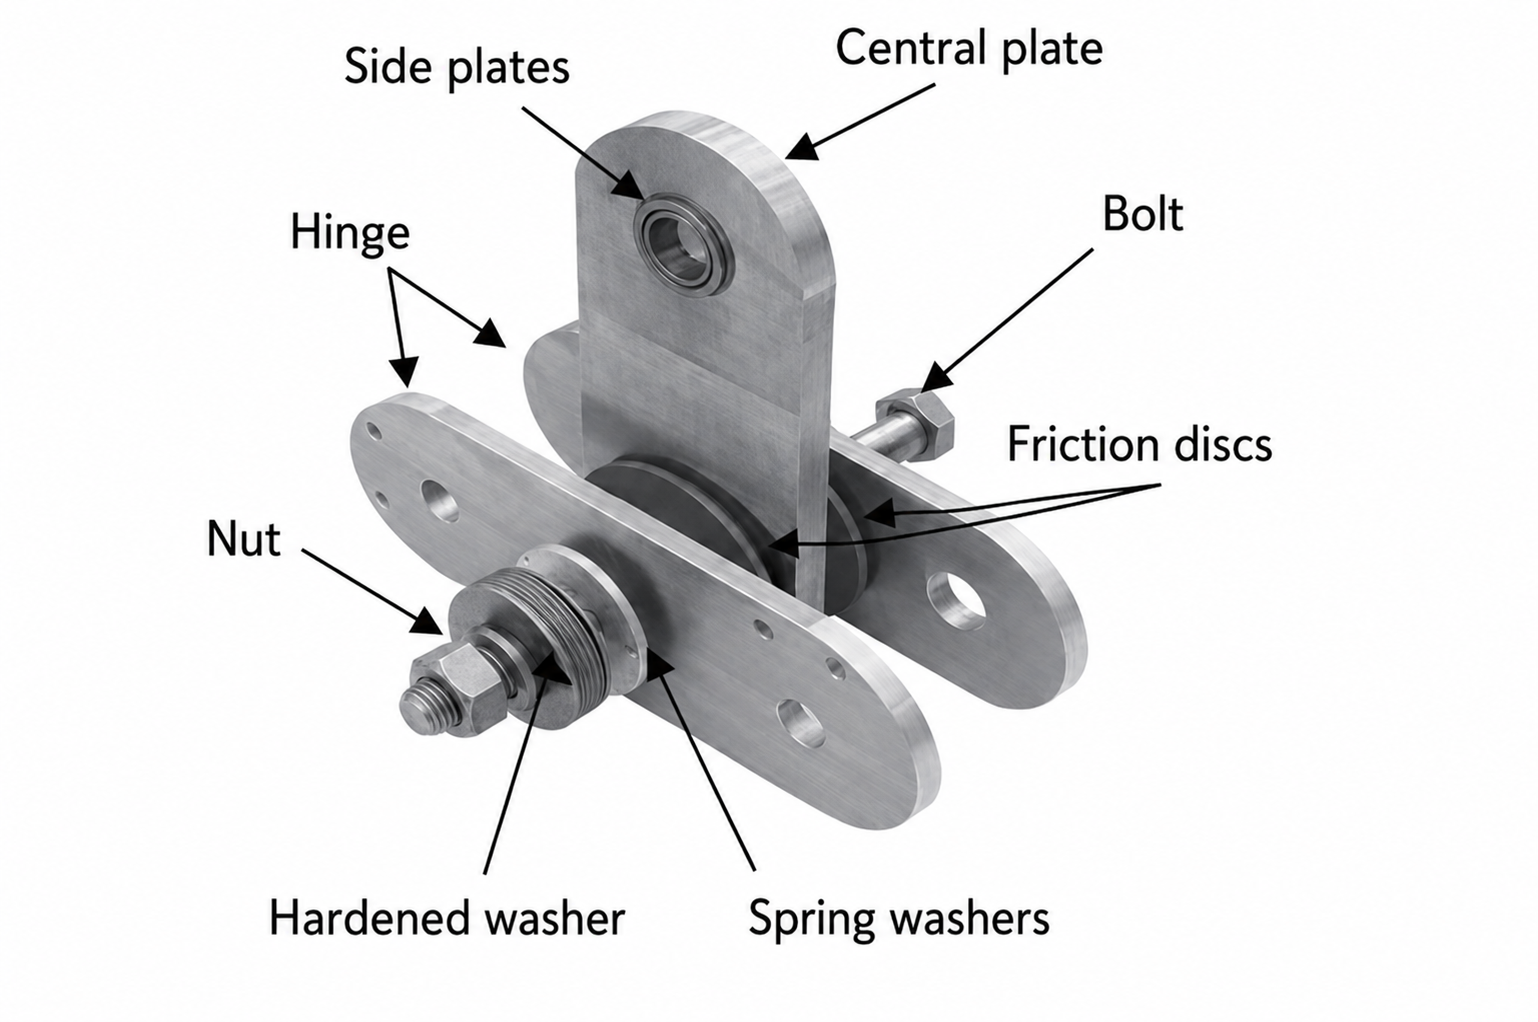
\includegraphics[width=\textwidth]{rfd_componentes.png}
    \end{subfigure}
    \hfill
    \begin{subfigure}[b]{0.48\textwidth}
        \centering
        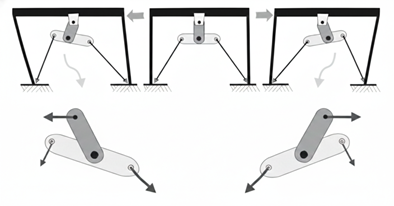
\includegraphics[width=\textwidth]{rfd_mecanismo.png}
    \end{subfigure}
    \caption{Rotational Friction Damper (RFD). The left panel shows the
             physical configuration of the device---central plate, side plates,
             friction discs, pre-tensioned bolt, and washers
             \citep{Mualla2002}---; the right panel illustrates the activation
             mechanism: lateral story drift induces rotation in the device,
             dissipating energy through friction.}
    \label{fig:rfd}
\end{figure}

\begin{figure}[htbp]
\centering
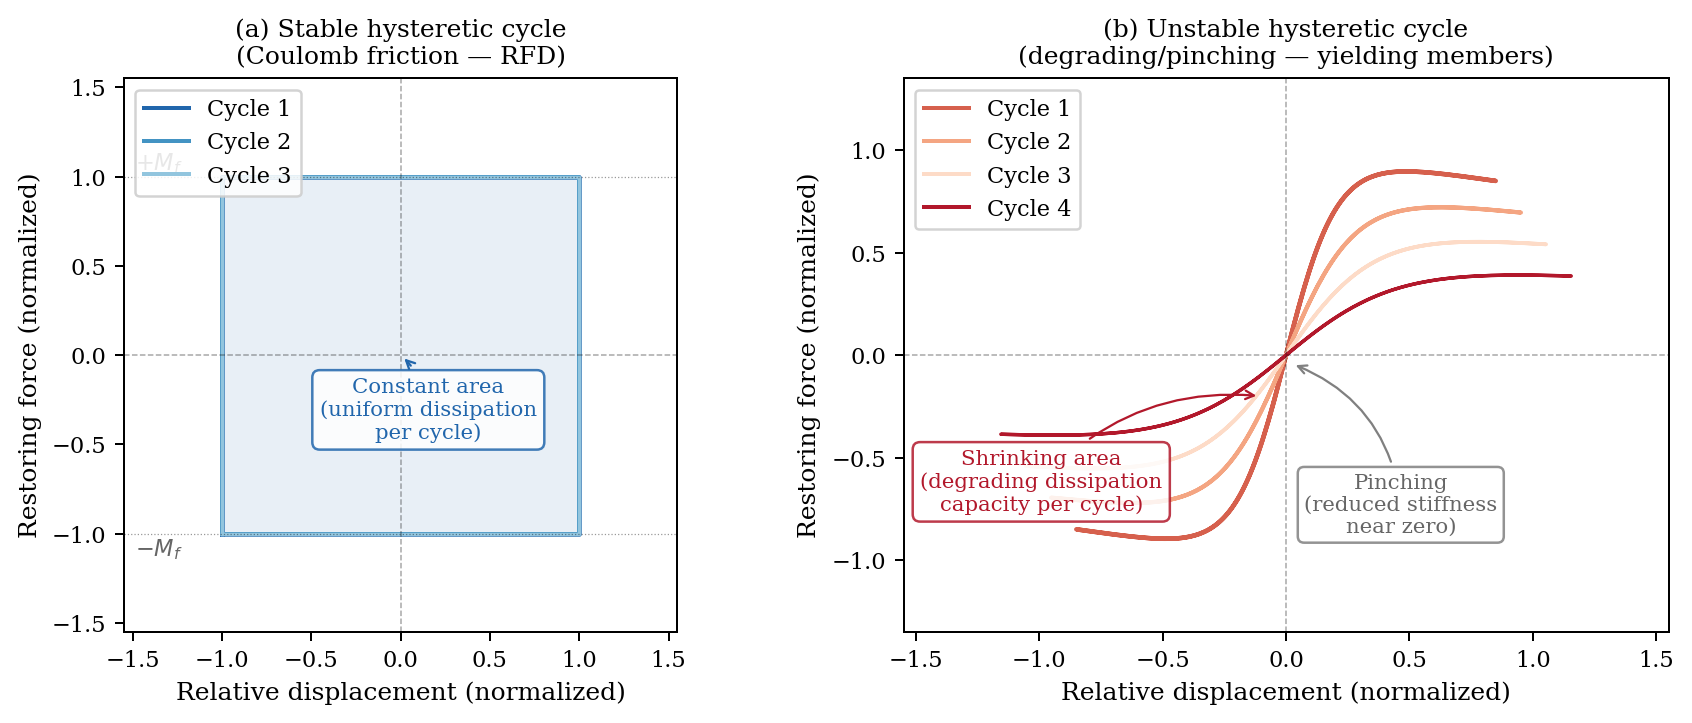
\includegraphics[width=\linewidth]{figs/F0_hysteresis_comparison.png}
\caption{Comparison of hysteretic cycle types in the force--displacement
plane. Panel~(a) shows the stable, rectangular cycle produced by Coulomb
friction (RFD): the enclosed area---equal to the dissipated energy---remains
constant across successive cycles because the friction mechanism does not
accumulate damage. Panel~(b) shows a degrading and pinching cycle typical of
yielding structural members: the area decreases with each cycle as strength
and stiffness deteriorate due to accumulated damage.}
\label{fig:histeresis}
\end{figure}

The central plate connects to the beam and the side plates to the brace.
When the frame drifts laterally during an earthquake, the relative inter-story
movement rotates the device and generates friction, transferring to the RFD
the energy that would otherwise damage the frame \citep{kim_use_2011}.

Capacity is expressed as the maximum friction moment $\Mf$. The equivalent
lateral force transmitted is:
\begin{equation}
    f_{\mathrm{RFD}} = \frac{\Mf}{\ha},
    \label{eq:Fafr}
\end{equation}
where $\ha$ is the brace lever arm. \citet{Mualla2002} verified that the
behavior is frequency-independent in the 2--7\,Hz range, justifying the use
of Coulomb's law.

\subsection{Dynamic Analysis with Non-Smooth Dynamics}
\label{sec:theory:dns}

Coulomb friction switches abruptly between slip and stick states, which
conventional time integrators handle poorly \citep{chopra_dynamics_2015}.
Two families of workarounds are common in the literature: regularization
approaches replace the discontinuous sign function with a smooth surrogate
(e.g., a bilinear or hyperbolic tangent approximation), and equivalent-damping
approaches substitute the friction device with a viscous dashpot of matched
energy dissipation \citep{lee_seismic_2025, Jarrahi2020jbe}. Both introduce
modeling error at the slip--stick transition and require case-specific
calibration, which becomes impractical at the scale of ${\approx}434{,}000$
simulations pursued here.

The Non-Smooth Dynamics (NSD) method of \citet{Namorado2022} avoids these
approximations entirely by reformulating the friction law as a
differential-algebraic inclusion and solving the resulting complementarity
problem at each timestep. This has two direct advantages for the present
study. First, \textit{theoretical fidelity}: the rectangular hysteretic loop
and the sharp slip--stick transitions of Coulomb friction are reproduced
exactly, without tuning parameters, ensuring that the dataset fed to the
ML models reflects the true nonlinear physics rather than a surrogate of a
surrogate. Second, \textit{computational scalability}: once the per-step
problem is cast as a Linear Complementarity Problem (LCP) solved with
Projected Successive Over-Relaxation (PSOR), each timestep requires only a
small number of sequential scalar updates (typically fewer than 20
iterations to convergence), making the method fast enough to be applied to
thousands of structural configurations without incurring the overhead of
general nonlinear solvers.

\subsubsection*{Friction law}

For an RFD between floors $i$ and $i+1$, the resisting moment follows
Coulomb's law:
\begin{equation}
    M_{\mathrm{RFD},i} \in -\Mf \cdot \operatorname{Sign}\!\left(\dot{\varphi}_i\right),
    \label{eq:coulomb}
\end{equation}
with the set-valued sign function:
\begin{equation}
    \operatorname{Sign}(v) =
    \begin{cases}
        \{+1\}    & \text{if } v > 0, \\
        [-1,\,+1] & \text{if } v = 0, \\
        \{-1\}    & \text{if } v < 0.
    \end{cases}
    \label{eq:sign}
\end{equation}
When the device slips, the moment equals $\pm\Mf$. At rest, it can take any
value in $[-\Mf,\,+\Mf]$ according to equilibrium.

\subsubsection*{Equation of motion}

The $\np$-story system with $n_a$ dampers follows the differential inclusion
\citep{Namorado2022}:
\begin{equation}
    \bm{M}\,\ddot{\bm{u}} + \bm{C}\,\dot{\bm{u}} + \bm{K}\,\bm{u}
    \in -\bm{M}\,\bm{r}\,\ddot{x}_g(t) + \bm{H}\,\bm{Q}_f(t),
    \label{eq:eom}
\end{equation}
where $\bm{M}$, $\bm{C}$, and $\bm{K}$ are the mass, damping, and stiffness
matrices; $\bm{u}$ is the ground-relative displacement vector; $\ddot{x}_g(t)$
is the ground acceleration; $\bm{r}$ is the seismic influence vector
(unit vector for a shear frame); $\bm{H}$ maps which floors contain dampers;
and $\bm{Q}_f(t)$ is the set-valued friction force vector arising from
Coulomb's law. In the discrete form, the set-valued force is
replaced by impulses $\bm{\lambda}_{k+1}$ computed at each step via a Linear
Complementarity Problem (LCP, Eq.~\ref{eq:lcp}):
\begin{equation}
    \bm{M}\,\ddot{\bm{u}} + \bm{C}\,\dot{\bm{u}} + \bm{K}\,\bm{u}
    = -\bm{M}\,\bm{r}\,\ddot{x}_g(t) + \bm{H}\,\bm{\lambda}_{k+1}/\Delta t.
    \label{eq:eom_disc}
\end{equation}

\subsubsection*{From Coulomb friction to a Linear Complementarity Problem}

The discrete equations of motion (Eq.~\ref{eq:eom_disc}) and Coulomb's law
(Eq.~\ref{eq:coulomb}) must be satisfied simultaneously at each timestep.
Jointly, they impose a condition on the friction impulse $\lambda_r$ of each
damper that cannot be expressed as a standard equation: at every step,
exactly one of two mutually exclusive physical states holds.

\begin{itemize}
    \item \textit{Slip state.} The contact surfaces are sliding. The impulse
    saturates at its physical bound, $|\lambda_r| = F^{\lim}_r \equiv
    \Mf\,\Delta t / \ha$, and the residual relative velocity at the device
    is nonzero, determined entirely by the structural motion.

    \item \textit{Stick state.} The contact is locked; the relative velocity
    at the device is zero. The impulse takes whatever value in
    $[-F^{\lim}_r,\,+F^{\lim}_r]$ is needed to enforce equilibrium, and
    it need not reach the bound.
\end{itemize}

This either/or structure---where a variable is either at its bound or the
associated constraint is active as an equality, but not both simultaneously---
is the defining property of a \textit{complementarity condition}. For the
bilateral (tension--compression symmetric) case arising from Coulomb friction,
finding the impulse vector $\bm{\lambda}$ that is consistent with both the
equations of motion and the friction law is therefore equivalent to solving
a Linear Complementarity Problem (LCP): find $\bm{\lambda}$ such that
\begin{equation}
    \bm{W}\bm{\lambda} + \bm{q} = \bm{0},
    \quad |\lambda_r| \leq F^{\lim}_r \equiv \frac{\Mf\,\Delta t}{\ha},
    \quad r = 1,\ldots,n_a.
    \label{eq:lcp}
\end{equation}
The matrix $\bm{W} \in \mathbb{R}^{n_a \times n_a}$ and the vector
$\bm{q} \in \mathbb{R}^{n_a}$ are assembled from the structural matrices
and the free-velocity predictor (Stage~1). Specifically,
$\bm{W} = (\bm{H}^{\top}\hat{\bm{M}}^{-1}\bm{H})\,\Delta t$ is the
\textit{compliance matrix} of the damper degrees of freedom: the diagonal
entry $W_{rr}$ is the local flexibility at device $r$ (how much a unit
impulse at $r$ changes the relative velocity at $r$ itself), and the
off-diagonal entry $W_{rs}$ quantifies the mechanical coupling between
devices $r$ and $s$ through the structure. The right-hand side $q_r$ is
the free inter-story relative velocity at device $r$, computed in Stage~1.
Solving the LCP means finding the impulse $\bm{\lambda}$ that, when applied
back to the structure, simultaneously brings all devices to their correct
state---slip or stick---in a globally consistent manner.

\subsubsection*{Solution by Projected Successive Over-Relaxation}

The LCP (Eq.~\ref{eq:lcp}) is solved iteratively with Projected Successive
Over-Relaxation (PSOR), a constrained extension of the classical
Gauss-Seidel method. The fundamental idea is to decompose the
$n_a$-dimensional problem into $n_a$ scalar sub-problems, each of which is
solved in closed form, and to enforce the Coulomb constraint immediately
after each update by projecting the result onto the admissible interval.

Each PSOR iteration cycles through the $n_a$ dampers in order. For damper
$r$, assuming all other impulses $\lambda_s^{(i)}$ ($s \neq r$) are fixed
at their current values, the $r$-th equation of the LCP can be solved
analytically to give the \textit{unconstrained} impulse:
\begin{equation}
    \tilde{\lambda}_r =
    -\frac{q_r + \displaystyle\sum_{s \neq r} W_{rs}\,\lambda_s^{(i)}}{W_{rr}}.
    \label{eq:gstep}
\end{equation}
This is the classical Gauss-Seidel step: it gives the exact solution for
$\lambda_r$ that satisfies the $r$-th row of the system if friction were
unconstrained. However, the result may violate the friction bound
$F^{\lim}_r$, so it is immediately projected onto the admissible interval:
\begin{equation}
    \lambda_r^{(i+1)} = \max\!\left(-F^{\lim}_r,\;\min\!\left(F^{\lim}_r,\;
    \tilde{\lambda}_r\right)\right).
    \label{eq:psor}
\end{equation}
The projection is the key step where the physical state of each device is
decided: if $|\tilde{\lambda}_r| > F^{\lim}_r$, the impulse is clamped to
the bound (the device is slipping); if $|\tilde{\lambda}_r| \leq F^{\lim}_r$,
the unconstrained value is accepted (the device is sticking). After the
projection, $\lambda_r^{(i+1)}$ immediately replaces $\lambda_r^{(i)}$
before moving to damper $r+1$. This \textit{successive} use of the most
recently updated values---as opposed to the \textit{simultaneous} update of
the Jacobi method---is what accelerates convergence.

Convergence of PSOR for this class of bilateral LCP is theoretically
guaranteed because $\bm{W}$ is positive semi-definite: it is a Gram-type
matrix $\bm{H}^{\top}\hat{\bm{M}}^{-1}\bm{H}$ scaled by $\Delta t$, and
$\hat{\bm{M}}^{-1}$ inherits the positive definiteness of the effective
mass matrix \citep{Namorado2022}. In practice, the iteration is initialized
with the warm-start $\bm{\lambda}^{(0)} = \bm{\lambda}_k$ (the solution
from the previous timestep), which exploits the temporal continuity of the
seismic response to reduce the number of iterations. Convergence is declared
when $\|\bm{\lambda}^{(i+1)} - \bm{\lambda}^{(i)}\|_\infty \leq 10^{-6}$,
with a safety cap of 20 iterations; in practice, fewer than five iterations
suffice for the vast majority of timesteps.

\subsubsection*{NSD-LCP-PSOR procedure}

The algorithm advances from step $k$ to $k+1$ in three stages; the complete
pseudocode is listed in Algorithm~\ref{alg:nsd-lcp-psor}. Before entering
the time loop, the matrices $\hat{\bm{M}}$, $\bm{A}$, and $\bm{W}$ are
computed once:
\begin{equation}
    \hat{\bm{M}} = \bm{M} + \theta\Delta t\,\bm{C} + (\theta\Delta t)^{2}\bm{K},
    \qquad
    \bm{A}       = \bm{M} - \theta\Delta t\,\bm{C} - (\theta\Delta t)^{2}\bm{K},
    \label{eq:Mhat}
\end{equation}
\begin{equation}
    \bm{W} = \left(\bm{H}^{\top}\hat{\bm{M}}^{-1}\bm{H}\right)\Delta t,
    \label{eq:W}
\end{equation}
and the initial conditions are set to
$\bm{u}_0 = \dot{\bm{u}}_0 = \bm{\lambda}_0 = \bm{0}$.

\textbf{Stage~1 — Free-velocity predictor.}
The velocity that the system would reach at step $k+1$ in the absence of
friction forces is computed as:
\begin{equation}
    \dot{\bm{u}}^{\mathrm{free}} = \hat{\bm{M}}^{-1}
    \!\left[
        \bm{A}\,\dot{\bm{u}}_k
        - \Delta t\,\bm{K}\bm{u}_k
        - \theta\Delta t\,\bm{M}\!\left(\ddot{x}_{g,k+1}+\ddot{x}_{g,k}\right)\bm{r}
    \right].
    \label{eq:vfree}
\end{equation}
The free inter-story relative velocity at each damper location $r$ is then:
\begin{equation}
    q_r = \dot{u}^{\mathrm{free}}_{f_r} - \dot{u}^{\mathrm{free}}_{f_r - 1},
    \qquad r = 1,\ldots,n_a,
    \label{eq:qr}
\end{equation}
where $f_r$ is the floor index of the $r$-th damper.

\textbf{Stage~2 — Friction corrector (LCP-PSOR).}
The vector $\bm{q}$ assembled in Stage~1 is used to form the LCP
(Eq.~\ref{eq:lcp}), which is solved with PSOR
(Eqs.~\ref{eq:gstep}--\ref{eq:psor}) as described in the preceding
subsection. The iteration is initialized with the warm-start
$\bm{\lambda}^{(0)} = \bm{\lambda}_k$ and yields the friction impulse
$\bm{\lambda}_{k+1}$ that simultaneously satisfies the equations of motion
and Coulomb's law.

\textbf{Stage~3 — State update.}
Once $\bm{\lambda}_{k+1}$ is known, the corrected velocity and displacement
at step $k+1$ are obtained by:
\begin{align}
    \dot{\bm{u}}_{k+1} &= \dot{\bm{u}}^{\mathrm{free}}
        + \Delta t\,\hat{\bm{M}}^{-1}\bm{H}\bm{\lambda}_{k+1}, \label{eq:vupdate}\\
    \bm{u}_{k+1} &= \bm{u}_k
        + \Delta t\!\left[(1-\theta)\,\dot{\bm{u}}_k
                         + \theta\,\dot{\bm{u}}_{k+1}\right]. \label{eq:uupdate}
\end{align}
The updated state $(\bm{u}_{k+1},\dot{\bm{u}}_{k+1})$ and impulse
$\bm{\lambda}_{k+1}$ are stored and the algorithm advances to step $k+2$.

\begin{algorithm}[t]
\caption{NSD-LCP-PSOR for multi-degree-of-freedom (MDOF) frames with RFDs}
\label{alg:nsd-lcp-psor}
\begin{algorithmic}[1]
\Require $\bm{M},\bm{C},\bm{K}$; $\bm{H}$, $\bm{F}^{\lim}$;
         $\{\ddot{x}_{g,k}\}_{k=0}^{n}$; $\Delta t$, $\theta$
\Ensure  $\{\bm{u}_k,\dot{\bm{u}}_k\}_{k=0}^{n}$
\vspace{2pt}
\State \textit{// Pre-computation (once)}
\State $\hat{\bm{M}} \leftarrow \bm{M} + \theta\Delta t\,\bm{C} + (\theta\Delta t)^{2}\bm{K}$
\State $\bm{A} \leftarrow \bm{M} - \theta\Delta t\,\bm{C} - (\theta\Delta t)^{2}\bm{K}$
\State $\bm{W} \leftarrow \left(\bm{H}^{\top}\hat{\bm{M}}^{-1}\bm{H}\right)\Delta t$
\State $\bm{u}_0 \leftarrow \bm{0}$;\quad $\dot{\bm{u}}_0 \leftarrow \bm{0}$;\quad
       $\bm{\lambda}_0 \leftarrow \bm{0}$
\vspace{2pt}
\For{$k = 0, 1, \ldots, n-1$}
    \State \textit{// Step 1 — free velocity}
    \State $\bm{b}_k \leftarrow \bm{A}\,\dot{\bm{u}}_k
            - \Delta t\,\bm{K}\bm{u}_k
            - \theta\Delta t\,\bm{M}\!\left(\ddot{x}_{g,k+1}+\ddot{x}_{g,k}\right)\bm{r}$
    \State $\dot{\bm{u}}^{\mathrm{free}} \leftarrow \hat{\bm{M}}^{-1}\bm{b}_k$
    \State \textit{// Step 2 — free relative velocities}
    \State $q_r \leftarrow \dot{u}^{\mathrm{free}}_{f_r} - \dot{u}^{\mathrm{free}}_{f_r-1}$
           \quad for $r = 1,\ldots,n_a$
    \State \textit{// Step 3 — PSOR corrector}
    \State $\bm{\lambda}^{(0)} \leftarrow \bm{\lambda}_k$
    \While{$\|\bm{\lambda}^{(i+1)} - \bm{\lambda}^{(i)}\|_\infty > \varepsilon$}
        \For{$r = 1,\ldots,n_a$}
            \State $\tilde{\lambda}_r \leftarrow
                   -\!\left(q_r + \sum_{s \neq r} W_{rs}\lambda_s^{(i)}\right)\!\big/W_{rr}$
            \State $\lambda_r^{(i+1)} \leftarrow
                   \max\!\left(-F^{\lim}_r,\;\min\!\left(F^{\lim}_r,\;\tilde{\lambda}_r\right)\right)$
        \EndFor
    \EndWhile
    \State $\bm{\lambda}_{k+1} \leftarrow \bm{\lambda}^{(*)}$
           \quad\textit{($F^{\lim}_r = \Mf\Delta t/\ha$)}
    \State \textit{// Step 4 — state update}
    \State $\dot{\bm{u}}_{k+1} \leftarrow
           \dot{\bm{u}}^{\mathrm{free}} +
           \Delta t\,\hat{\bm{M}}^{-1}\bm{H}\bm{\lambda}_{k+1}$
    \State $\bm{u}_{k+1} \leftarrow \bm{u}_k +
           \Delta t\!\left[(1-\theta)\,\dot{\bm{u}}_k +
                           \theta\,\dot{\bm{u}}_{k+1}\right]$
\EndFor
\end{algorithmic}
\end{algorithm}

The time step $\Delta t = 0.01$\,s matches the sampling interval of the
seismic records, avoiding interpolation. For the stiffest structures
($T_1 = 0.3$\,s), this gives 30 points per period, satisfying the criterion
$\Delta t / T_1 \leq 0.10$ \citep{chopra_dynamics_2015}. The friction force
at floor $i$ is:
\begin{equation}
    f_{\mathrm{RFD},i} = \frac{\lambda_i}{\ha\,\Delta t}.
    \label{eq:ffrict}
\end{equation}

\subsubsection*{Extension of the NSD method to large-scale MDOF simulation}

The method of \citet{Namorado2022} was validated for frames of one to five
stories. The NSD-LCP-PSOR implementation developed here was previously
verified in \citet{Ponce2026} for a 10-story shear frame subjected to five
real seismic records under a Monte Carlo probabilistic framework, confirming
hysteretic cycles and displacement responses consistent with the literature.
Three adaptations were made to extend the method to frames of up to twenty
stories.

\textbf{Joint LCP.} The impulses of all dampers are solved simultaneously
using the matrix $\bm{W}$, which captures how the devices interact through
the structure.

\textbf{No tuning parameter.} The original algorithm requires a case-specific
parameter $\alpha$. Formulating the problem as an LCP eliminates this
parameter, facilitating application to thousands of configurations.

\textbf{Warm start.} The impulse from the previous step serves as the initial
guess, reducing iterations because the response changes little between steps.

\subsection{Seismic Performance Metric}
\label{sec:theory:metrica}

Several metrics have been used in the literature to assess the effectiveness
of friction dampers. Energy-based criteria---such as the ratio of dissipated
energy to input energy adopted by \citet{Jarrahi2020jbe, Jarrahi2020sdee}---
measure how much of the seismic input is absorbed by the devices but do not
directly reflect the structural demands experienced by the building or its
occupants. Inter-story drift ratio is widely used for structural safety
assessment \citep{chopra_dynamics_2015}, but ignores floor accelerations,
which govern damage to non-structural components and equipment. Peak absolute
acceleration alone does not capture displacement response. Single-criterion
metrics therefore risk optimizing one demand parameter at the expense of
others: a configuration that reduces displacement but amplifies floor
accelerations---a known trade-off in passive control---would appear favorable
under drift-only criteria while being detrimental under a broader assessment.

To address this, the present study adopts the composite normalized index
$CR_2$, which simultaneously integrates the three engineering demand
parameters most relevant to building performance: peak displacement ($R_1$,
governing structural safety and residual drift), peak absolute acceleration
($R_2$, governing non-structural damage and occupant comfort), and peak base
shear ($R_3$, governing foundation demands). Normalizing each component by
the corresponding uncontrolled response makes $CR_2$ dimensionless and
directly comparable across the 1,000 structures analyzed, regardless of
their height, mass, or stiffness. The relationship between $CR_2$ and the
energy-based threshold of \citet{Jarrahi2020sdee} is discussed in
\cref{sec:discussion}.

The performance of each configuration is measured by normalized ratios with
respect to the uncontrolled structure
\citep{Namorado2022, Jarrahi2020jbe, Mualla2002}:
\begin{equation}
    R_1 = \frac{u_{\max}^{(\mathrm{c})}}{u_{\max}^{(0)}}, \quad
    R_2 = \frac{\ddot{u}_{\max}^{(\mathrm{c})}}{\ddot{u}_{\max}^{(0)}}, \quad
    R_3 = \frac{V_{\max}^{(\mathrm{c})}}{V_{\max}^{(0)}},
    \label{eq:R_individual}
\end{equation}
where superscript (c) denotes the controlled structure and (0) the
uncontrolled one. Two composite indices are formed:
\begin{equation}
    CR_1 = \sqrt{R_1^2 + R_2^2}, \qquad
    CR_2 = \sqrt{R_1^2 + R_2^2 + R_3^2}.
    \label{eq:CR}
\end{equation}
Without dampers, $CR_2 = \sqrt{3}$; lower values indicate improvement.
Because $CR_2$ depends on the record, it is summarized over the eight
accelerograms with three statistics \citep{Kazemi2022}:
\begin{align}
    \CR{P10} &= Q_{0.10}\!\left(\{CR_2^{(k)}\}_{k=1}^{N_r}\right), \quad
    \CR{med}  = Q_{0.50}\!\left(\{CR_2^{(k)}\}_{k=1}^{N_r}\right), \notag\\
    \CR{P90} &= Q_{0.90}\!\left(\{CR_2^{(k)}\}_{k=1}^{N_r}\right).
    \label{eq:CR2stats}
\end{align}
where $Q_p(\cdot)$ denotes the $p$-th sample quantile and $N_r = 8$ is the
number of seismic records. The subscript stands for percentile (P).

The choice of these three statistics is grounded in both statistical and
engineering reasoning. From a statistical standpoint, with $N_r = 8$ records
the 10th and 90th percentiles correspond approximately to the 1st and 7th
ranked values of the ordered sample---that is, to the record that excites
the structure least effectively and the one that excites it most effectively
within the available ensemble. They therefore define the practical extremes
of record-to-record variability without being sensitive to a single outlier.
The median ($Q_{0.50}$) provides the central estimate, robust to the
asymmetry that often characterizes $CR_2$ distributions.

From an engineering standpoint, this three-statistic summary is consistent
with the multi-stripe analysis framework recommended by FEMA~P-58
\citep{FEMAP58} and adopted in recent seismic performance studies
\citep{Kazemi2022}: low percentiles represent seismic conditions favorable
to the damper (low-intensity or spectrally mismatched records where the
uncontrolled structure also performs well), while high percentiles represent
conservative conditions where demand is large and every unit of additional
control capacity matters. Accordingly, $\CR{P10}$ is interpreted as the
\emph{favorable} scenario, $\CR{med}$ as the \emph{typical} scenario, and
$\CR{P90}$ as the \emph{conservative} scenario throughout this study.
The ratio $\CR{P90}/\CR{P10}$ serves as a measure of design robustness:
configurations for which this ratio is close to unity perform consistently
across the record ensemble, while high ratios signal sensitivity to
ground-motion selection.

\subsection{Machine Learning for Structural Optimization}
\label{sec:theory:ml}

The goal is to learn a continuous mapping from design variables to seismic
performance so that the response surface can be explored without running
additional simulations. Because $CR_2$ is a real-valued engineering demand
parameter rather than a class label, this is inherently a regression
problem: a function $\hat{y} = f(\bm{x};\,\bm{\theta})$ is trained to
predict each $CR_2$ statistic from the structural and damper configuration
$\bm{x}$. Training minimizes the mean squared error (MSE):
\begin{equation}
    \mathcal{L}(\bm{\theta}) = \frac{1}{N}\sum_{i=1}^{N}
    \bigl(y_i - f(\bm{x}_i;\,\bm{\theta})\bigr)^2.
    \label{eq:mse}
\end{equation}

The three targets---$\CR{P10}$, $\CR{med}$, and $\CR{P90}$---are predicted
by independent models rather than a single multi-output model. This choice is
deliberate: each percentile represents a structurally different relationship
between design variables and seismic response. The 10th percentile captures
favorable ground motion conditions, where a few critical decisions dominate;
the median reflects typical seismic demand, governed by a broader set of
variables; the 90th percentile represents the conservative scenario, where
placement and friction moment effects are partially diluted by high input
energy. Because these relationships differ, a shared model would
systematically underfit at least one target. Independent models allow each
to specialize in the structure of its own response surface, as confirmed by
the divergent feature importance rankings in \cref{sec:results:importancia}.

Four algorithms are compared, deliberately spanning a complexity range from
simple to complex. Linear Regression and Ridge Regression
\citep{Hastie2009} serve as linear baselines: strong baseline performance
would imply that the design space is approximately linear and a response
surface could be characterized with far fewer simulations; poor performance
reveals genuine nonlinearity---a conclusion that cannot be drawn without the
comparison. Random Forest \citep{Breiman2001} introduces nonlinearity and
interaction effects by averaging $n = 100$ trees trained on bootstrap
replicates of the data. XGBoost \citep{Chen2016} builds trees sequentially,
each correcting the residuals of its predecessors. The contrast between
these two ensemble strategies is itself informative: boosted models tend to
outperform when errors are structured (systematic functions of the input),
while bagged models are more robust when errors are closer to noise.

A critical methodological challenge arises from the experimental design: each
of the 1,000 structures contributes approximately 50 RFD configurations, so
the same structure appears in many rows. Splitting data randomly would allow
structure-specific patterns---eigenfrequency, mass distribution, stiffness
profile---to appear in both training and validation folds, artificially
inflating apparent generalization. To prevent this data leakage,
generalization is assessed with five-fold GroupKFold
cross-validation \citep{Kazemi2022}, with groups defined by structure
identifier: all configurations of a given structure are always assigned to
the same fold, ensuring the model is evaluated on structures it has never
seen during training. This protocol measures the ability to generalize to new
structures---the operationally relevant condition for a design-support tool.

The two evaluation metrics are the cross-validated Root Mean Square Error
($\mathrm{RMSE_{CV}}$) and the cross-validated coefficient of determination
($R^2_{\mathrm{CV}}$), where the subscript stands for cross-validated (CV),
indicating that both quantities are averaged over the five GroupKFold folds:
\begin{equation}
    \RMSE = \sqrt{\frac{1}{|V|}\sum_{i \in V}\bigl(y_i - \hat{y}_i\bigr)^2},
    \qquad
    \Rsq  = 1 - \frac{\sum_{i \in V}(y_i - \hat{y}_i)^2}
                      {\sum_{i \in V}(y_i - \bar{y})^2},
    \label{eq:metrics}
\end{equation}
where $V$ is the validation fold, $|V|$ its cardinality, $\hat{y}_i$ are
out-of-fold predictions, and $\bar{y}$ is the sample mean of $y_i$ over
$V$. Beyond predictive accuracy, feature importance from XGBoost---measured
as the mean decrease in impurity (MDI) aggregated across all trees---ranks
the contribution of each design variable to each target, providing
interpretable design guidance: variables with high importance identify the
dimensions of the design space where engineering decisions have the greatest
leverage on seismic performance.

%%═══════════════════════════════════════════════════════════════════════════
\section{Methodology}
\label{sec:method}
%%═══════════════════════════════════════════════════════════════════════════

\subsection{Design of Experiments}
\label{sec:method:doe}

To obtain conclusions that generalize across the building stock rather than
for a single structure, 1,000 shear-type frames were generated by a
randomized Latin Hypercube Sampling \citep[LHS;][]{McKay1979} design,
implemented via \texttt{scipy.stats.qmc.LatinHypercube}
\citep{Virtanen2020}. In this variant, the range of each factor is divided
into $N$ equal-probability strata and exactly one sample is drawn from each
stratum after a random intra-stratum permutation; the scramble step
preserves uniform marginal coverage while reducing point clustering and
improving the low-discrepancy properties of the design without assuming any
functional form of the response. Each frame is defined by five factors: the
number of stories $\np \in \{3, 5, 7, 10, 12, 15, 18, 20\}$, chosen to
span low- to high-rise typologies; the fundamental period
$T_1 \in [0.3,\,3.0]$\,s; the mean floor mass
$\bar{m} \in [150,\,350]$\,t; a mass profile (uniform, linearly increasing,
decreasing, or concentrated at the top); and a stiffness profile (uniform,
linearly increasing, decreasing, or soft-story at the base). Stiffness
vectors were calibrated analytically by iteratively scaling $\bm{k}$ until
the solution of the eigenvalue problem
$(\bm{K} - \omega_1^2\,\bm{M})\,\bm{\phi}_1 = \bm{0}$ matched the target
period within $1\,\%$, where $\omega_1 = 2\pi/T_1$ and $\bm{\phi}_1$ is
the first mode shape.

For each structure, approximately 50 RFD configurations were generated to
cover the design space of damper placement and friction moment: 10
deterministic configurations targeting specific coverage levels (single
floor, all floors, upper half, lower half, and combinations thereof) to
anchor the extremes of the placement space, and 40 additional configurations
drawn by LHS over the binary placement space with $\Mf \in [25,\,500]$\,kN$\cdot$m
to explore the interior. The presence of an RFD at floor $i$ is encoded
as $b_i \in \{0,1\}$, giving a total damper count
$\nd = \|\bm{b}\|_0$ and a coverage density $\etad = \nd/\np$. Combined
with the eight seismic records applied to each configuration, the full
experimental plan comprises 433,984 time-history simulations.

\begin{figure}[htbp]
\centering
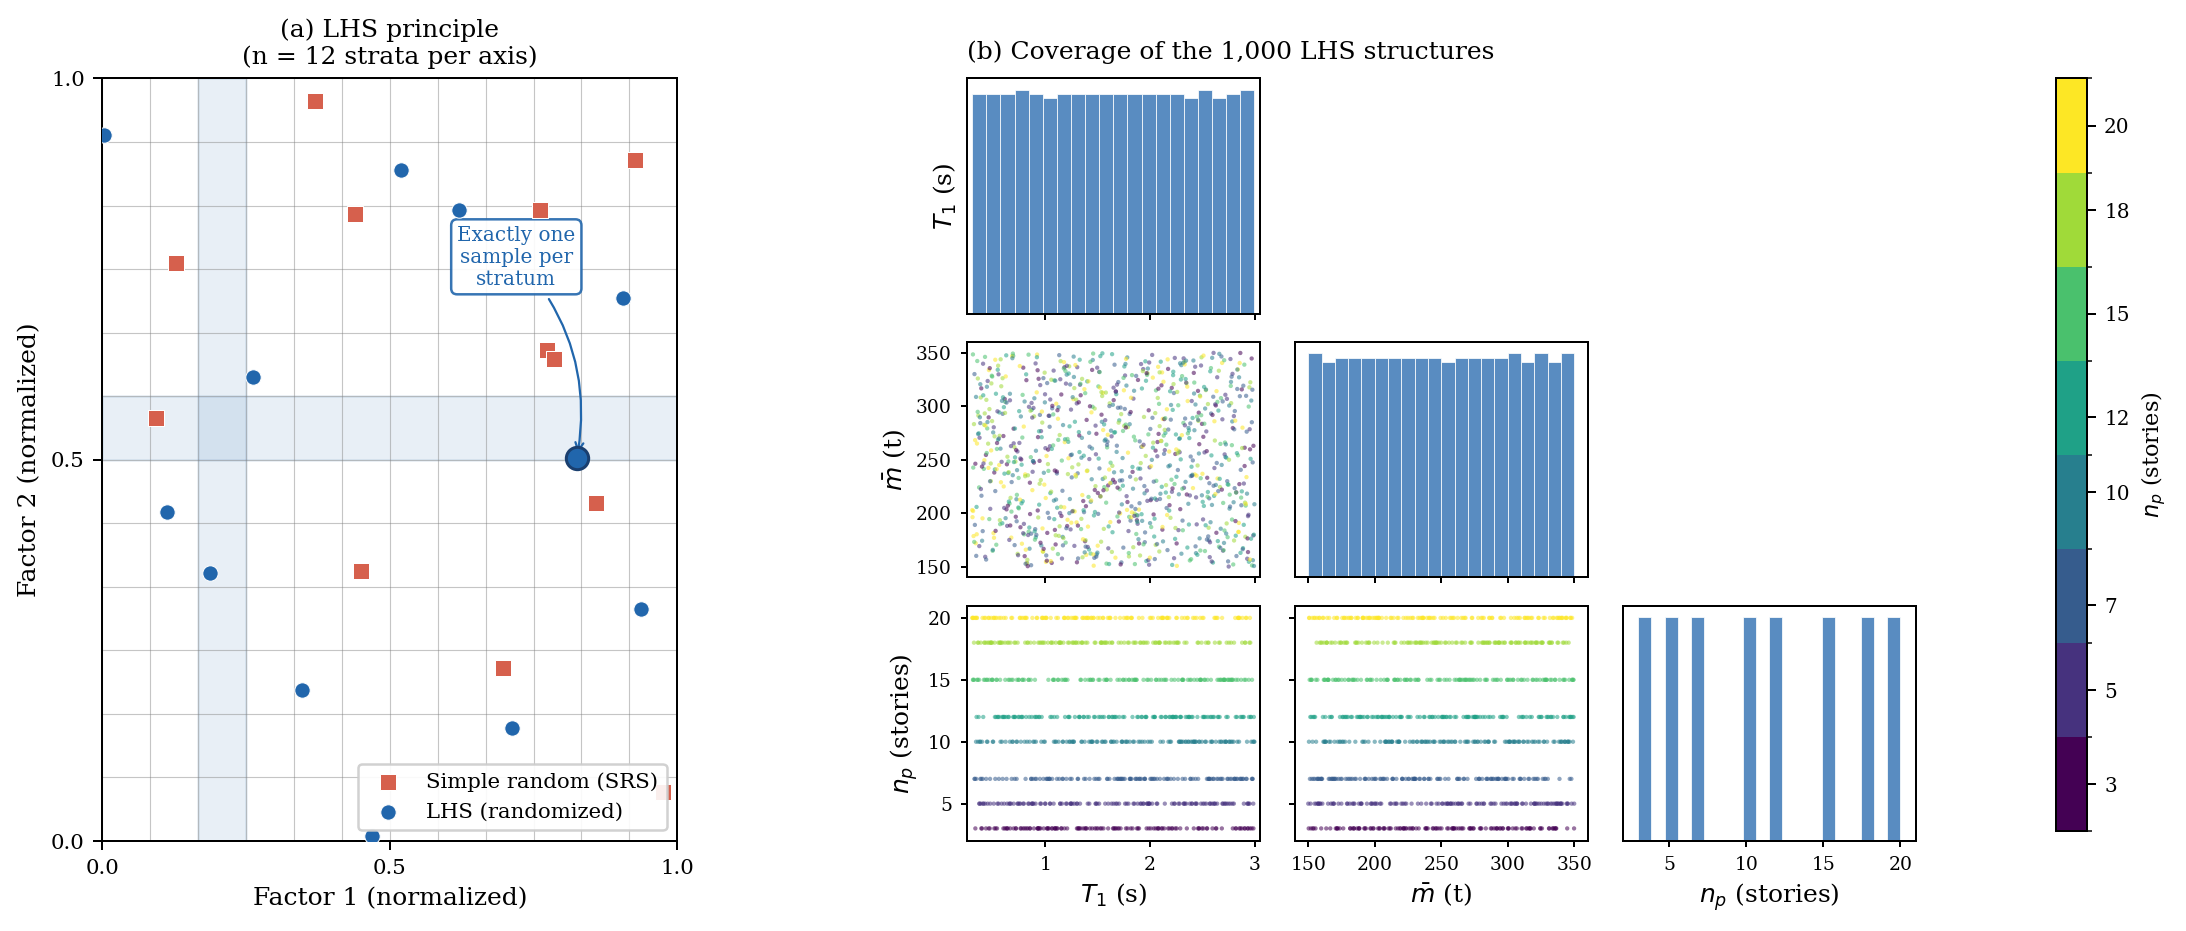
\includegraphics[width=\linewidth]{figs/F_LHS_design.png}
\caption{Latin Hypercube Sampling design used to generate the 1,000
structural models. Panel (a) illustrates the stratification principle for
two factors with $n = 12$ strata: unlike simple random sampling (red
squares), LHS (blue circles) places exactly one point per stratum along
each axis, guaranteeing uniform marginal coverage. Panel (b) shows the
actual coverage of the 1,000 generated structures projected onto the three
continuous design factors ($T_1$, $\bar{m}$, $n_p$); the diagonal panels
display the marginal histograms, confirming the near-uniform coverage
achieved by the randomized LHS design.}
\label{fig:lhs_design}
\end{figure}

\subsection{Structural Models and Dynamic Analysis}
\label{sec:method:modelo}

Each of the 1,000 frames is modeled as a linear shear frame with lumped
floor masses, an appropriate simplification for the parametric scope of this
study: the focus is on the effect of RFD placement and friction moment, not
on nonlinear structural behavior, so keeping the frame elastic isolates the
damper's contribution to the response \citep{chopra_dynamics_2015}. Inherent
structural damping is represented by Rayleigh damping with $\zeta = 3\,\%$,
calibrated to modes 1 and 3, a level consistent with lightly damped steel
moment-resisting frames \citep{chopra_dynamics_2015}.

Seismic excitation is applied through eight historical accelerograms selected
to span a wide range of frequency content, duration, and geographic origin:
El~Centro~1940, Kobe~1995, Northridge~1994, Loma~Prieta~1989,
Zacatula~1997, Jamiltepec~2018, Niltepec~2017, and Trinidad~1983. Using
multiple records rather than a single design spectrum is essential here: a
single record would bias the performance ranking of damper configurations
toward the frequency content of that specific event, while the ensemble of
eight records---and the subsequent percentile aggregation into $\CR{P10}$,
$\CR{med}$, and $\CR{P90}$---captures the variability of the seismic
environment. Each simulation runs with a time step of $\Delta t = 0.01$\,s
using the NSD-LCP-PSOR integrator described in \cref{sec:theory:nsd}, with
RFD lever arm $\ha = 0.40$\,m \citep{Mualla2002, Jarrahi2020jbe}.
All records were applied at their original, unscaled historical intensities;
no spectral matching or amplitude scaling was performed. As a result, $CR_2$
quantifies relative performance under the actual intensity of each historical
event rather than under a uniform hazard level, and cross-record comparisons
should be interpreted accordingly.

\subsection{Feature Engineering}
\label{sec:method:features}

The raw design variables $(\np, T_1, \Mf, \nd)$ characterize the structure
and the number of dampers, but say nothing about \emph{where} the dampers
are placed---a spatial dimension that may be decisive for performance. To
bridge this gap, five derived features are constructed to encode placement
geometry explicitly, and 20 binary indicators $b_1,\ldots,b_{20}$ provide
the full floor-level detail. Together, these form an input vector of 29
predictors that gives the model simultaneous access to global structural
properties, aggregate placement statistics, and fine-grained device location:

\begin{enumerate}[label=\textit{\roman*})]
    \item \textbf{Primary design variables} (4):
          $\np$, $T_1$, $\Mf$, and $\nd$.

    \item \textbf{Derived features} (5):
    \begin{itemize}
        \item $\etad = \nd/\np$: coverage density, the ratio of instrumented
              floors to total stories---the dominant predictor, as shown in
              \cref{sec:results:importancia};
        \item $\bar{p} = \tfrac{1}{\nd}\sum_{i:\,b_i=1} i$: mean damper
              position (floor index);
        \item $\tilde{p} = \bar{p}/\np$: normalized mean position, making
              $\bar{p}$ comparable across buildings of different height;
        \item $\sigma_p = \mathrm{std}\!\left(\{i:b_i=1\}\right)/\np$:
              normalized vertical dispersion, distinguishing clustered from
              spread configurations with the same $\nd$;
        \item $\tilde{E} = E_{\mathrm{total}}/(\np\times10^6)$: total
              dissipated energy normalized per floor, a simulation-derived
              feature that partly reflects the interaction between
              placement and structural response.
    \end{itemize}

    \item \textbf{Binary placement indicators} (20):
          $b_i = 1$ if floor $i$ carries an RFD, zero otherwise; frames
          with fewer than 20 stories are zero-padded so the input dimension
          is constant across the dataset.
\end{enumerate}

\subsection{Training and Validation}
\label{sec:method:entrenamiento}

Following the framework established in \cref{sec:theory:ml}, the three
targets are predicted by independent models. For each target, all four
algorithms are trained on the same 29,000-configuration dataset and evaluated
under the same GroupKFold protocol, making comparisons between models
directly meaningful. Hyperparameters were fixed at widely used defaults to
avoid overfitting the model selection process: Random Forest uses $n = 100$
trees with maximum depth 15; XGBoost uses $n = 100$ estimators, a maximum
tree depth of 6, and a learning rate of $\eta = 0.1$; Ridge Regression uses
$\alpha = 1.0$. No tuning was performed on the validation folds, ensuring
that reported metrics reflect genuine out-of-sample performance.

Feature importance was extracted from the trained XGBoost model using the
mean decrease in impurity (MDI) criterion: at each internal split of each
tree, the improvement in MSE weighted by the number of samples reaching that
node is attributed to the splitting feature, and these values are averaged
across all 100 trees. Because MDI can be influenced by high-cardinality
features, the binary placement indicators $b_i$ are each relatively sparse;
their individual importances are reported alongside the derived aggregates
($\etad$, $\bar{p}$, $\sigma_p$) to allow comparison between floor-level
detail and summary statistics. The ranking is computed separately for each
target, exposing the differences in variable relevance across seismic
percentiles discussed in \cref{sec:results:importancia}.

%%═══════════════════════════════════════════════════════════════════════════
\section{Results}
\label{sec:results}
%%═══════════════════════════════════════════════════════════════════════════

\subsection{Predictive Performance of the ML Models}
\label{sec:results:desempenio}

The central question at this stage is whether the seismic performance of RFD
configurations can be predicted accurately enough to serve as a surrogate for
simulation, and whether the design space is linear or fundamentally nonlinear.
\Cref{tab:desempenio} reports the cross-validated $\RMSE$ and $\Rsq$ for each
model–target combination, and the answer to both questions is unambiguous.
Ensemble methods outperform linear baselines by a wide margin: XGBoost reduces
$\RMSE$ by 49\,\% relative to Ridge for $\CR{med}$ and by 40\,\% for
$\CR{P10}$, achieving $\Rsq = 0.920$ and $\Rsq = 0.933$, respectively
(\cref{fig:comparacion_modelos}). This performance gap is not a modeling
artifact---it is a direct signal that the relationship between design variables
and seismic performance is genuinely nonlinear, with interaction effects that
no linear model can capture.

\begin{table}[h!]
\centering
\caption{Cross-validated RMSE and $R^2$ by model and target variable.
         Five-fold GroupKFold, grouped by structure identifier.}
\label{tab:desempenio}
\small
\setlength{\tabcolsep}{4pt}
\begin{tabular}{lcccccc}
\toprule
& \multicolumn{2}{c}{$\CR{med}$}
& \multicolumn{2}{c}{$\CR{P10}$}
& \multicolumn{2}{c}{$\CR{P90}$} \\
\cmidrule(lr){2-3}\cmidrule(lr){4-5}\cmidrule(lr){6-7}
Model & $\RMSE$ & $\Rsq$ & $\RMSE$ & $\Rsq$ & $\RMSE$ & $\Rsq$ \\
\midrule
Linear Regression & 0.1274 & 0.695 & 0.1267 & 0.812 & 0.1838 & 0.435 \\
Ridge             & 0.1274 & 0.695 & 0.1268 & 0.812 & 0.1838 & 0.435 \\
Random Forest     & 0.0681 & 0.913 & 0.0785 & 0.928 & 0.0981 & \textbf{0.839} \\
XGBoost           & \textbf{0.0652} & \textbf{0.920} & \textbf{0.0755} & \textbf{0.933} & 0.0984 & 0.838 \\
\bottomrule
\end{tabular}
\end{table}

\begin{figure}[htbp]
\centering
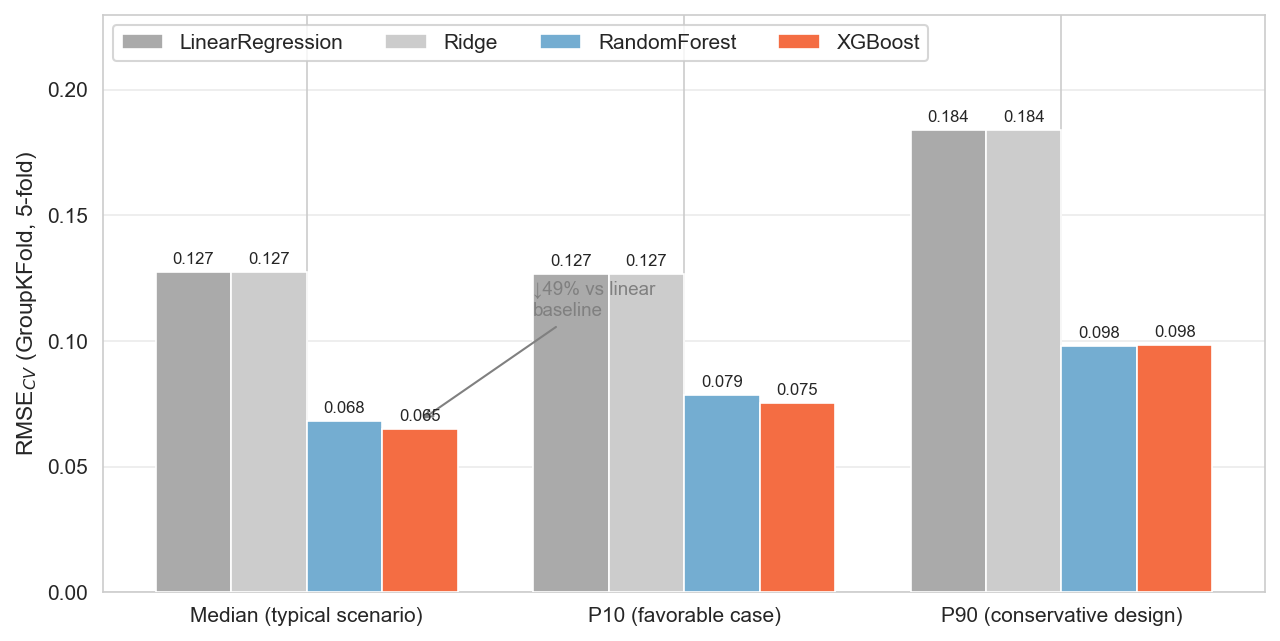
\includegraphics[width=0.85\linewidth]{figs/F1_model_comparison_rmse.png}
\caption{Cross-validated $\RMSE$ comparison across models and target
variables. Ensemble models achieve approximately half the error of the
linear baselines.}
\label{fig:comparacion_modelos}
\end{figure}

The degree of nonlinearity, however, is not uniform across the three targets.
For $\CR{P10}$---the favorable seismic scenario---linear models already reach
$\Rsq = 0.81$, suggesting that under moderate excitation the dominant
dependencies are approximately monotonic and the design space is relatively
smooth. The conservative scenario $\CR{P90}$ tells a sharply different story:
linear models collapse to $\Rsq = 0.44$, while Random Forest recovers
$\Rsq = 0.839$. Under the most demanding records, threshold effects and
placement interactions become decisive, and only tree-based models are
flexible enough to learn them. The slight advantage of Random Forest over
XGBoost for $\CR{P90}$ ($\Rsq = 0.839$ vs.\ $0.838$) is consistent with
this interpretation: bagging is more robust when the signal is partially
obscured by high-energy, record-specific variability.

\Cref{fig:pred_vs_actual} confirms that XGBoost predictions are unbiased
across the full range of $CR_2$: out-of-fold points track the identity line
without systematic deviation. The only region of elevated residuals is
$CR_2 > 1.8$, which corresponds exclusively to low-rise frames
($\np \leq 5$). In these structures, each damper affects a larger fraction
of the lateral system and the response is more sensitive to small parameter
variations---a regime that is inherently harder to predict but also represents
configurations of limited practical interest, since high $CR_2$ values indicate
poor damper effectiveness regardless of the model.

\begin{figure}[htbp]
\centering
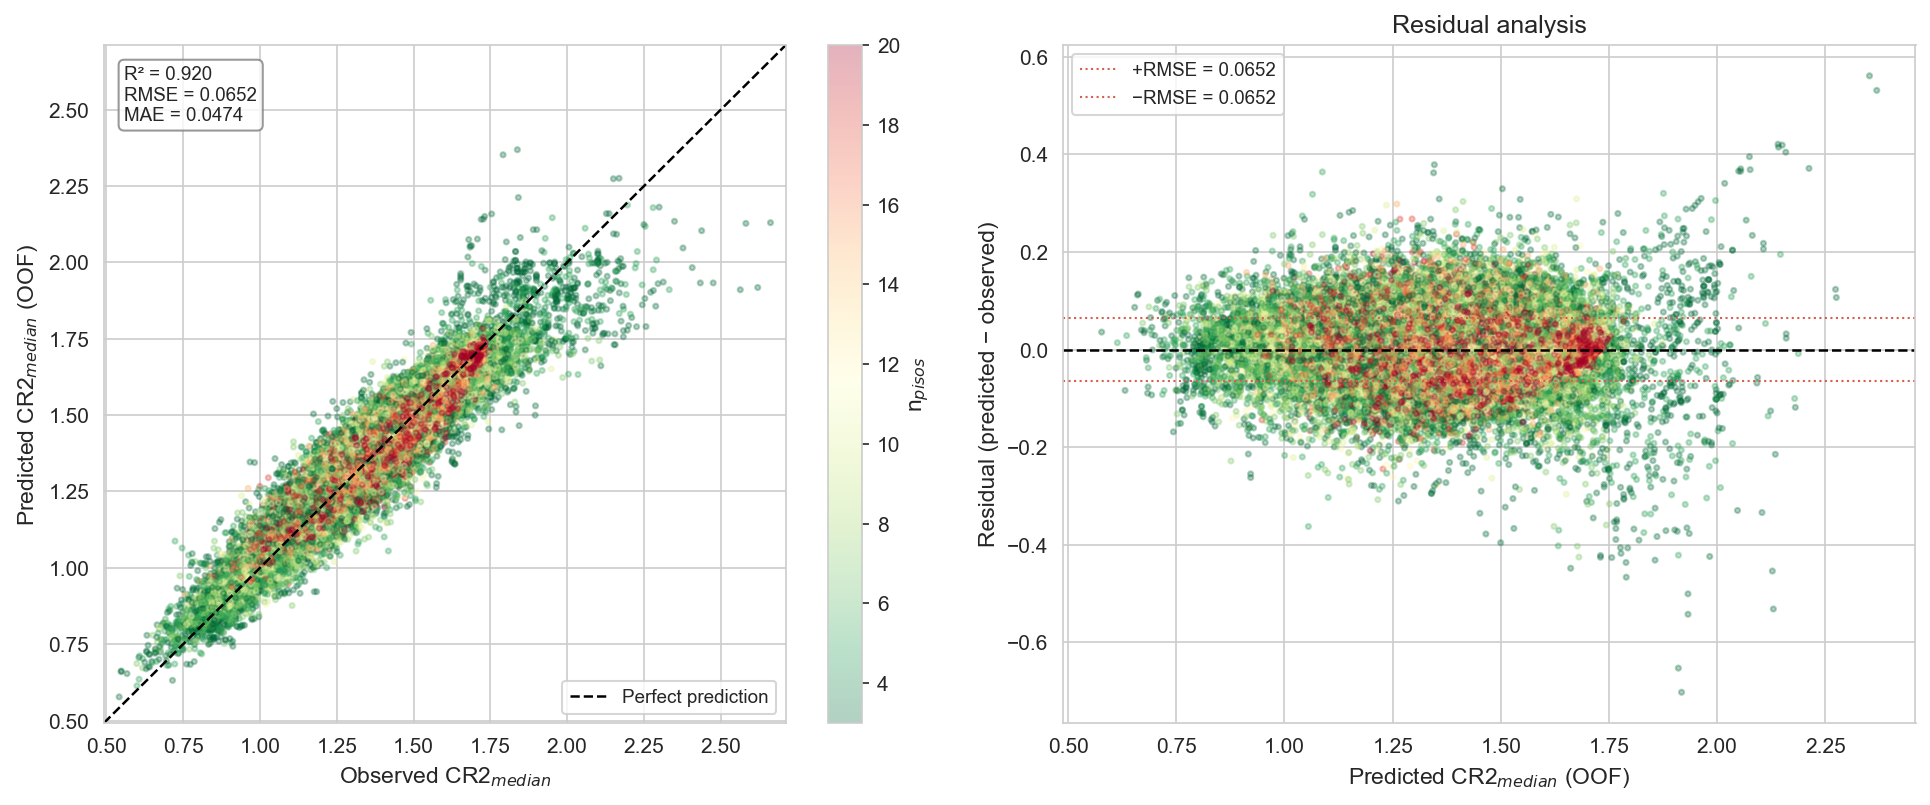
\includegraphics[width=\linewidth]{figs/F2_predicted_vs_actual_oof.png}
\caption{Out-of-fold performance of the XGBoost model for the typical seismic
scenario ($\CR{med}$, $\Rsq = 0.92$, $\RMSE = 0.065$). The left panel shows
predicted versus observed values, colored by number of stories~$\np$; the
right panel shows residuals versus predicted values, with $\pm\RMSE$ reference
bands.}
\label{fig:pred_vs_actual}
\end{figure}

\begin{figure}[htbp]
\centering
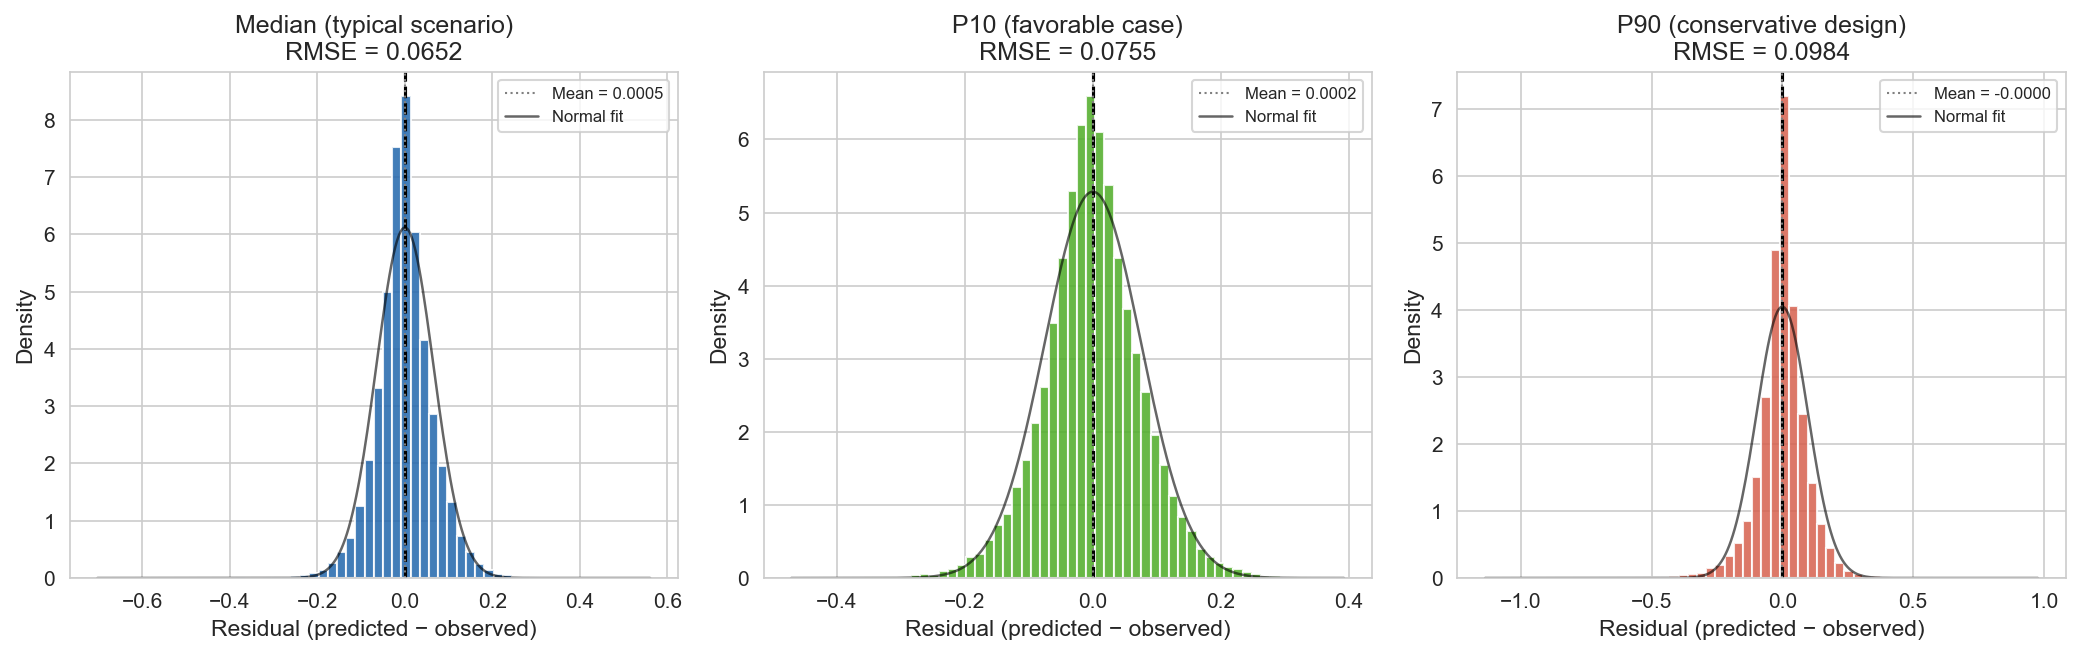
\includegraphics[width=\linewidth]{figs/F3_residual_distributions.png}
\caption{Residual distributions (out-of-fold, XGBoost) for the three $CR_2$
targets. Dashed line: zero mean; solid curve: normal fit.}
\label{fig:residuales}
\end{figure}

\subsection{Feature Importance and Variable Hierarchy}
\label{sec:results:importancia}

Understanding which design variables govern seismic performance is as
important as prediction accuracy: it translates a black-box model into
actionable engineering guidance. \Cref{fig:importancia} shows the 12 most
important predictors for each target according to the XGBoost MDI ranking.
The result is consistent and striking---coverage density $\etad$ ranks first
across all three scenarios, with a Pearson correlation of $\rho = -0.73$
with $\CR{med}$, far above the raw device count $\nd$ ($\rho = -0.45$).
This separation is meaningful: two structures with the same number of dampers
but different heights have very different $\etad$, and the one with higher
coverage consistently performs better. The MDI ranking captures this
nonlinear interaction directly, whereas a simple correlation analysis of
$\nd$ would have missed it.

Although dissipated energy $\tilde{E}$ achieves a similar Pearson correlation
($\rho = -0.70$), XGBoost assigns it a lower rank than $\etad$ across all
targets. This is expected: $\tilde{E}$ is itself a product of the simulation
and therefore partially encodes the structural response rather than being an
independent design input. Its high correlation is informative, but using it
as a predictor in a design context requires first running the simulation---
precisely what the surrogate model is meant to avoid. $\etad$, by contrast,
is known at the design stage. Vertical dispersion $\sigma_p$ ($\rho = -0.54$)
ranks third, reflecting the well-established finding that distributing devices
uniformly along the height promotes more homogeneous inter-story dissipation,
with the lower floors being particularly effective given their larger drift
demands \citep{aydin_simple_2013, moghaddam_optimal_2022,
miguel_simultaneous_2016}. Friction moment $\Mf$ shows weak marginal
correlation ($\rho = -0.19$) but interacts significantly with $\etad$, as
discussed in \cref{sec:results:interaccion}.

The importance hierarchy shifts in a revealing way for the conservative
scenario $\CR{P90}$: $\etad$ drops to fourth place, displaced by the binary
placement indicators for floors~1 and~2 and by frame height $\np$. Under the
most demanding records, global coverage is a necessary but insufficient
condition for good performance---the precise positioning of dampers at the
critical lower levels becomes the deciding factor. This shift has a direct
design implication: a conservative design strategy should prioritize lower
floors before adding coverage to upper ones.

\begin{figure}[htbp]
\centering
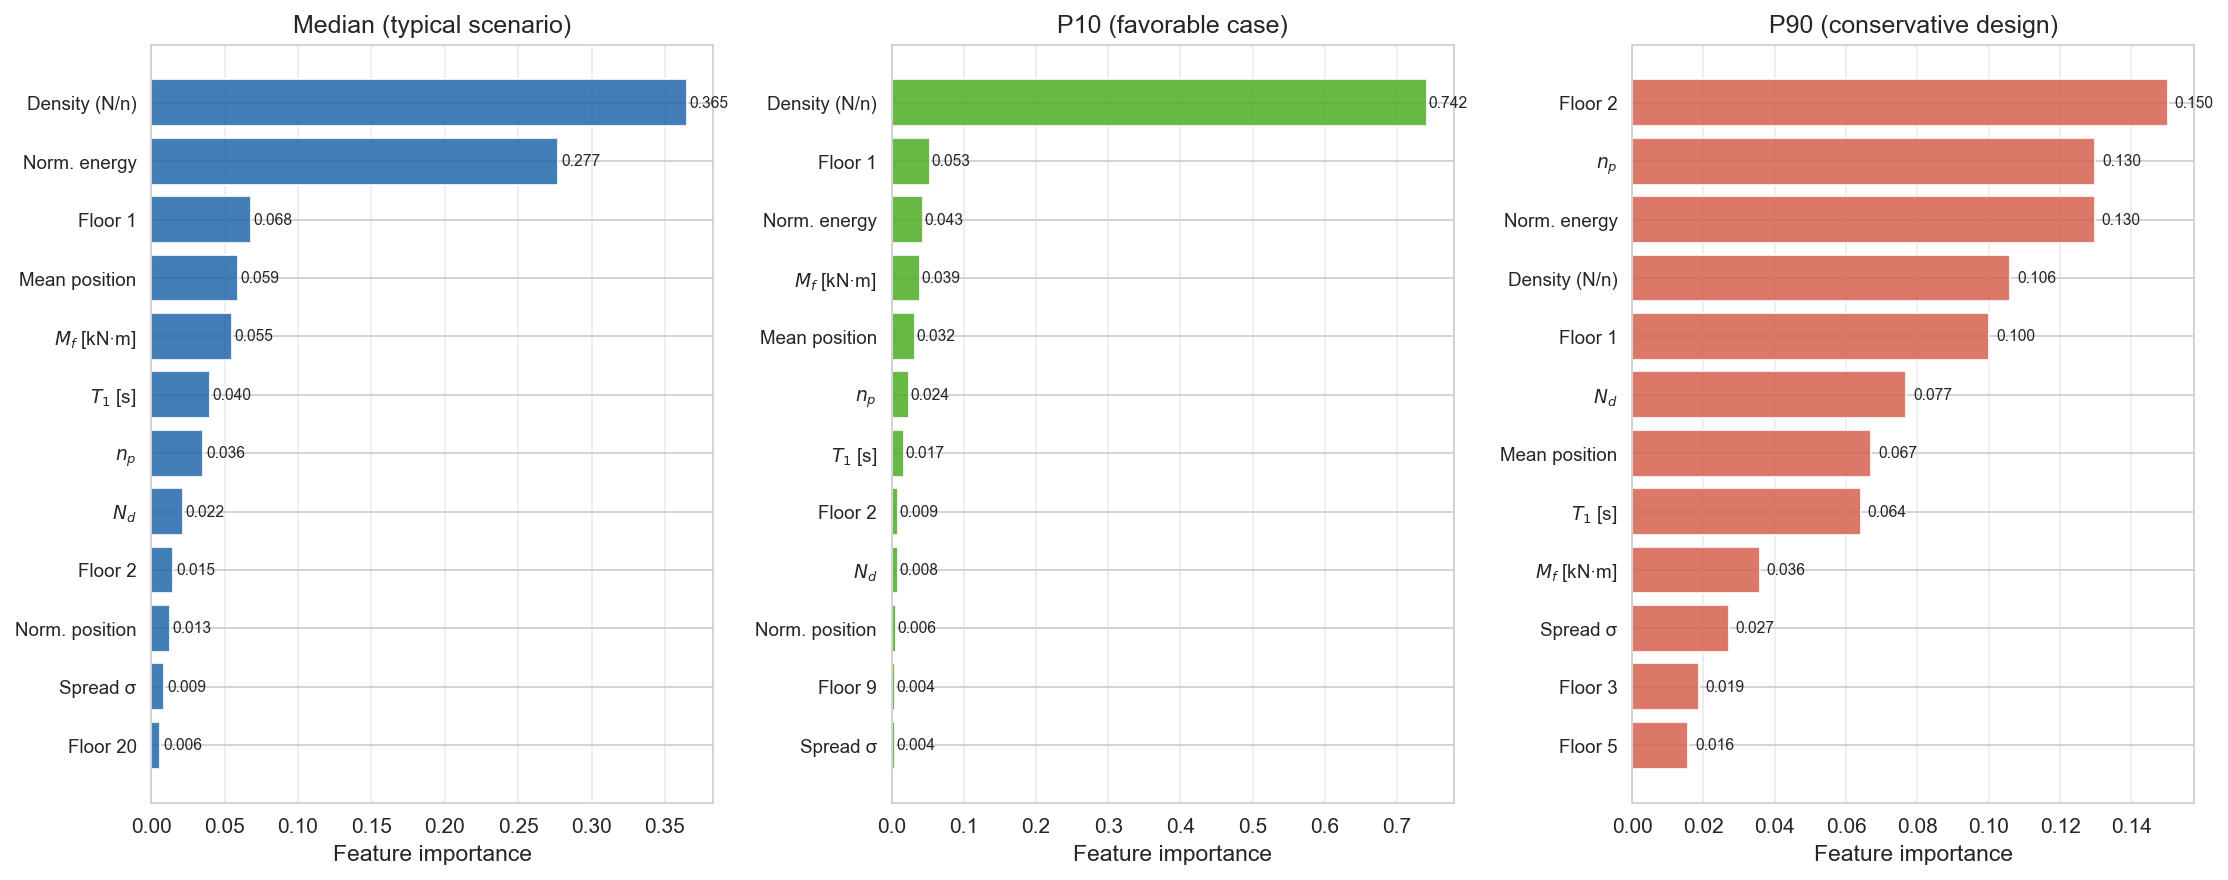
\includegraphics[width=\linewidth]{figs/F4_feature_importance_3targets.png}
\caption{Ranked feature importance of the XGBoost model for each of the three
design targets. The top-12 predictors are shown per scenario; horizontal scales
are independent across panels and should be compared by rank rather than by
absolute magnitude.}
\label{fig:importancia}
\end{figure}

\subsection{Diminishing Returns: Effect of Damper Coverage Density}
\label{sec:results:decreciente}

Knowing that $\etad$ is the dominant predictor raises a practical question:
how much coverage is enough? \Cref{fig:decreciente} shows the best achievable
$\CR{med}$ as a function of $\etad$, stratified by building height.
The relationship is consistently nonlinear across all height groups: gains are
largest in the range $\etad \in [0.30,\,0.60]$ and taper off progressively
beyond that point. To quantify the saturation objectively, a threshold was
defined as the coverage density at which 80\,\% of the maximum achievable
gain is reached. Mid- and high-rise frames (6--20 stories) cross this
threshold at $\etad \approx 0.85$, while low-rise frames (3--5 stories)
require $\etad \approx 0.95$ because each device covers a larger fraction of
the lateral system and removes a larger fraction of the remaining improvement
potential. The within-structure curves (\cref{fig:curvas_internas}) confirm
that this pattern is consistent across individual structures, not just at the
group level.

A potential confound in this analysis is that structures with higher $\etad$
may also differ systematically in $\Mf$, placement geometry, or building
height, so that the observed relationship reflects those variables rather than
coverage alone. To rule this out, a stochastic dominance test was applied
across the eight seismic records: the 5th percentile of $CR_2$ in each
density interval was compared against the 95th percentile of the immediately
lower interval. Dominance is confirmed for seven of the eight records,
meaning that even a configuration unfavorable in $\Mf$ or placement but with
higher coverage outperforms 95\,\% of lower-density configurations.
Record-wise Pearson correlations range from $\rho = -0.74$ (El~Centro~1940)
to $\rho = -0.55$ (Kobe~1995), confirming the robustness of the finding.
The sole exception is Trinidad~1983 ($\rho = -0.18$): the relatively
low-intensity spectral content of this record reduces inter-story drift demand
to a level where placement and per-device friction capacity recover importance
relative to global coverage---a physical result consistent with the role of
$\etad$ as a demand-driven variable.

\begin{figure}[htbp]
\centering
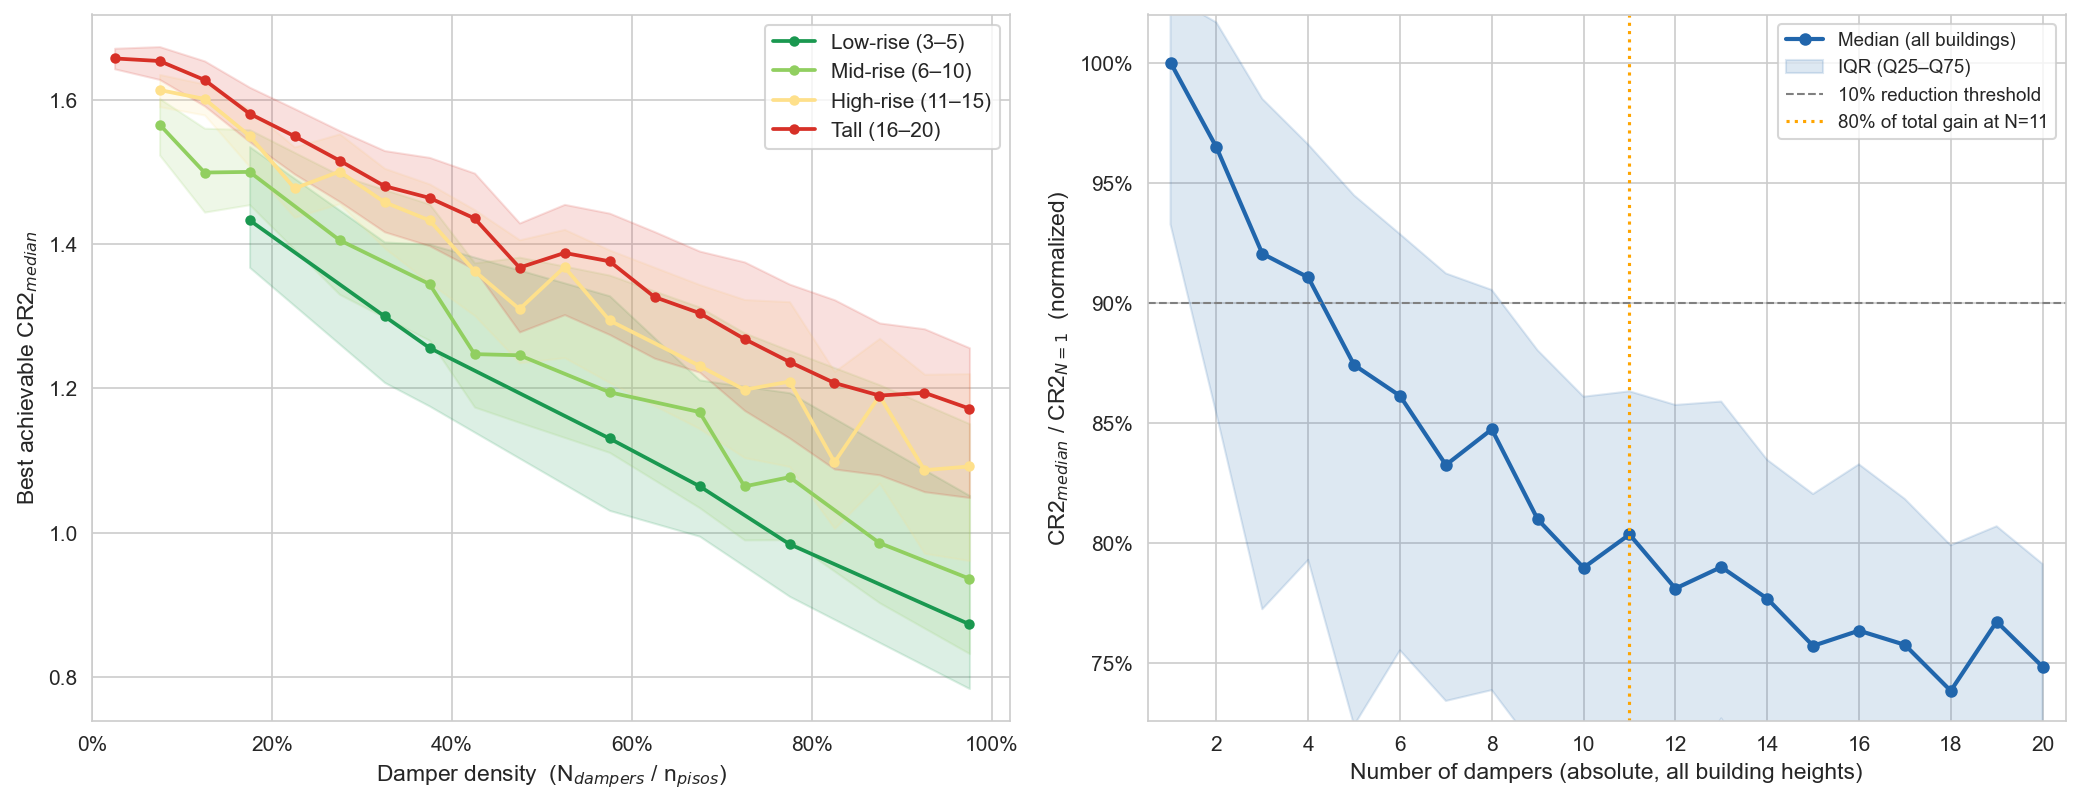
\includegraphics[width=\linewidth]{figs/F5_diminishing_returns.png}
\caption{Diminishing returns in seismic performance as a function of coverage
density $\etad = \nd/\np$, stratified by building height. Each curve shows
the best achievable $\CR{med}$ (minimum over all configurations at that
density), with the shaded band representing the interquartile range (IQR)
across structures in each height group.}
\label{fig:decreciente}
\end{figure}

\begin{figure}[htbp]
\centering
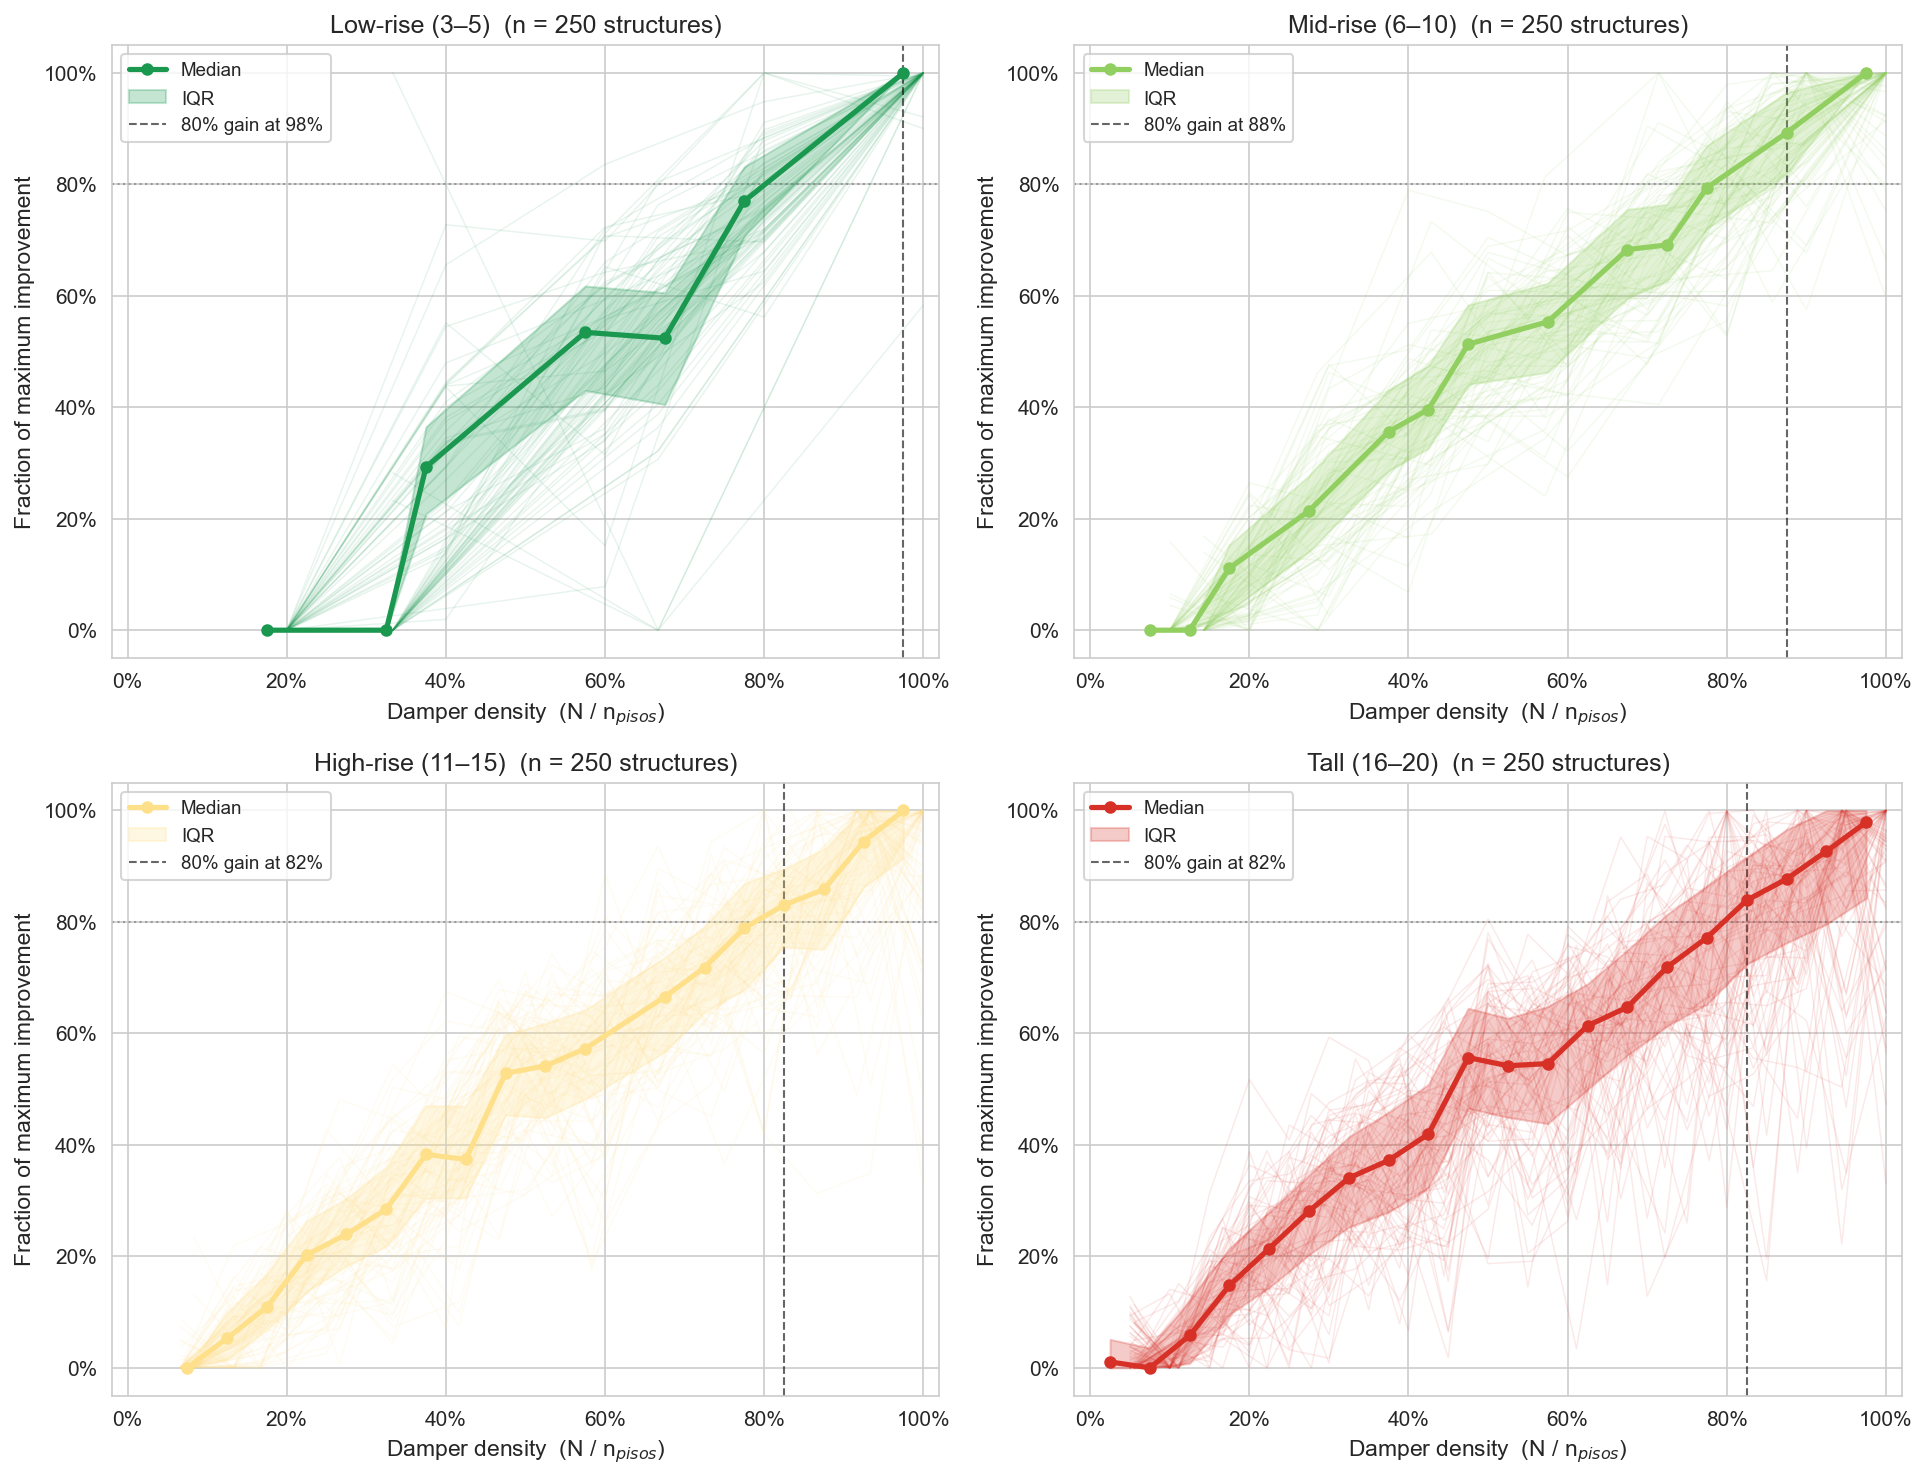
\includegraphics[width=\linewidth]{figs/F6_within_structure_curves.png}
\caption{Within-structure diminishing-returns curves. Each thin line is one
structure; the thick line is the median $\pm$ IQR. Dashed line: density at
which 80\,\% of the maximum gain is reached.}
\label{fig:curvas_internas}
\end{figure}

\subsection{Interaction Between Damper Count and Friction Moment}
\label{sec:results:interaccion}

While coverage density governs the first-order response, the friction moment
$\Mf$ is not a free parameter that can be set arbitrarily once coverage is
decided. \Cref{fig:mapa_calor} makes this interaction explicit: it maps
median $CR_2$ over a grid of binned $\nd$ and $\Mf$ values, stratified by
building height, revealing how the two variables reinforce or limit each other.

The clearest pattern across all height groups is that low coverage combined
with low friction ($\Mf \leq 100$\,kN$\cdot$m) consistently produces the
worst performance, while high coverage with moderate-to-high friction
approaches the optimum. The nature of the interaction, however, changes with
height. In low-rise frames (3--5 stories), $\nd$ and $\Mf$ contribute
approximately equally: increasing $\nd$ from 1--2 to 3--4 reduces $CR_2$
from 1.46 to 1.12, and increasing $\Mf$ from 100 to 300\,kN$\cdot$m yields
a comparable improvement at any fixed $\nd$. In mid- and high-rise frames,
the picture shifts: $\nd$ becomes the dominant lever, but $\Mf$ retains a
significant and consistent effect. Even at full coverage ($\nd \geq 11$), the
gap between $\Mf < 100$\,kN$\cdot$m and $\Mf > 400$\,kN$\cdot$m amounts to
0.46~$CR_2$ units in mid-rise frames. This confirms that $\Mf$ and $\nd$
are complementary, not substitutes: one cannot compensate for the other.

Optimal configurations across the dataset concentrate in the range
$\Mf \in [300,\,460]$\,kN$\cdot$m (median 400\,kN$\cdot$m,
IQR~[269,\,456]\,kN$\cdot$m) with coverage fractions close to unity,
providing a practical operating window for initial device sizing.

\begin{figure}[htbp]
\centering
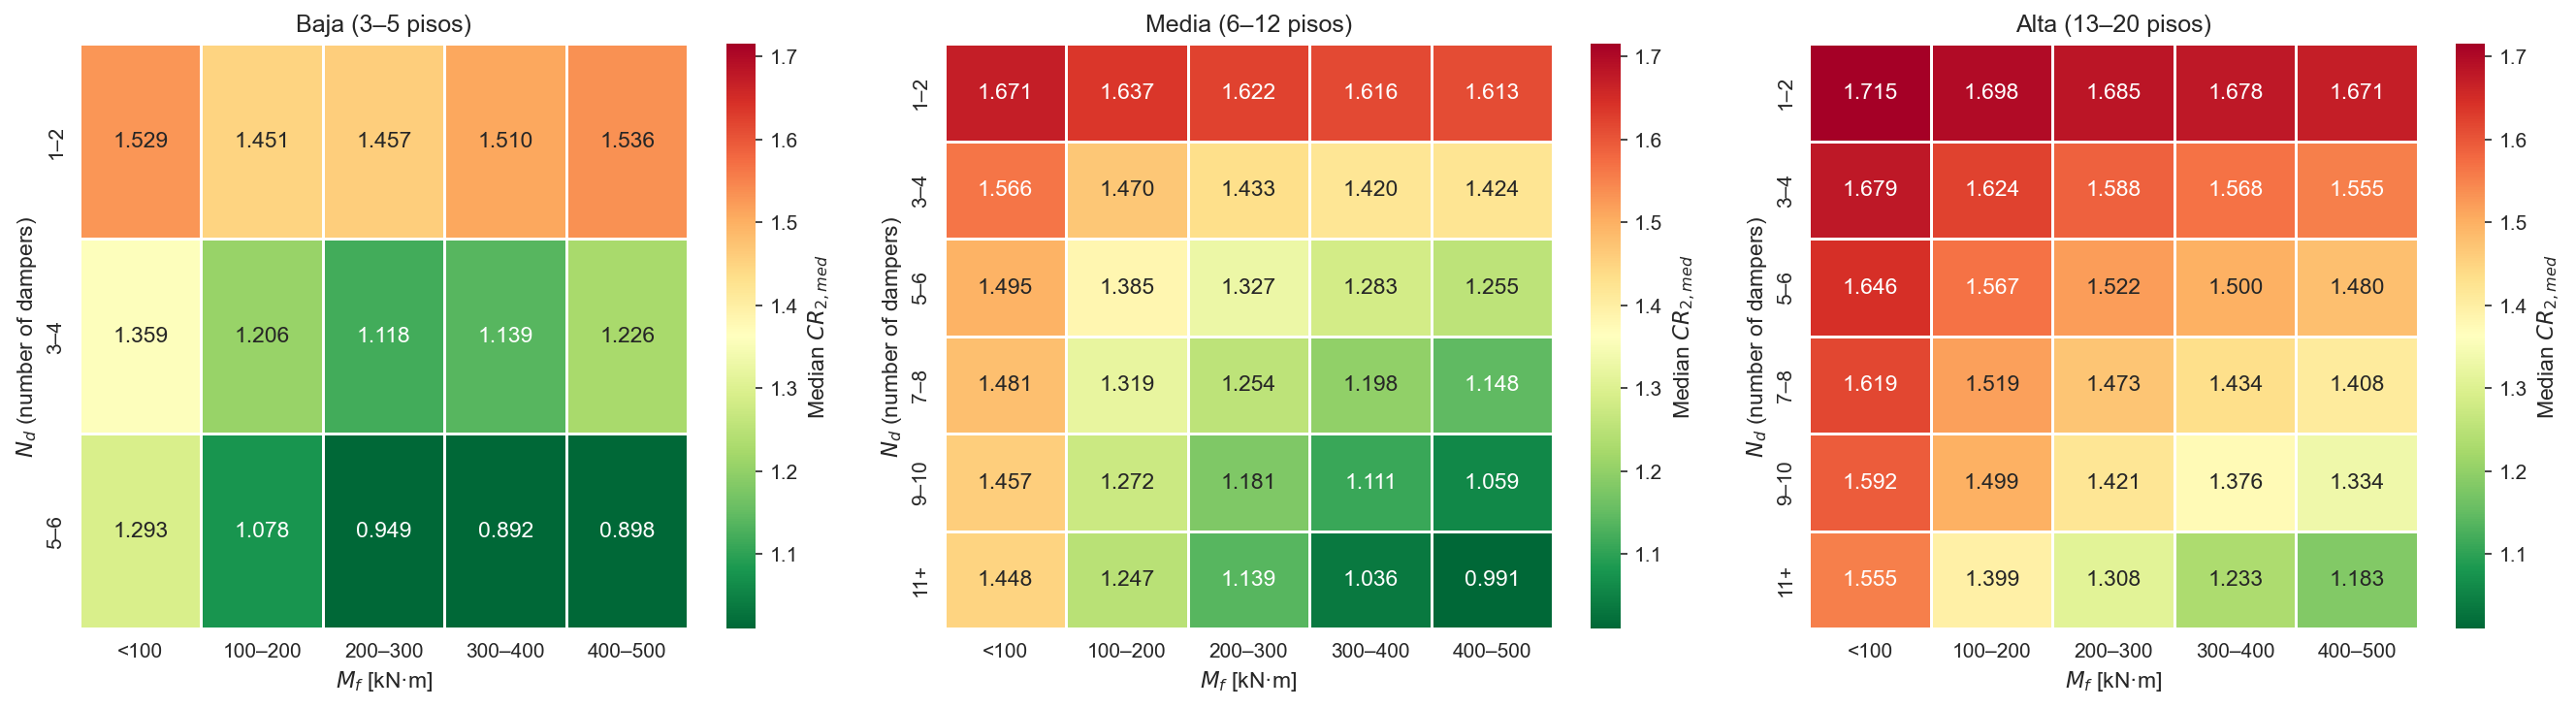
\includegraphics[width=\linewidth]{figs/F7_interaction_heatmap.png}
\caption{Median $CR_2$ as a function of binned $\nd$ and $\Mf$ (kN$\cdot$m),
stratified by building height: low-rise (3--5), mid-rise (6--12), and
high-rise (13--20 stories). Consistent color scale across panels.}
\label{fig:mapa_calor}
\end{figure}

\subsection{Design Convergence Across Seismic Scenarios}
\label{sec:results:convergencia}

A key practical question is whether the optimal number of dampers changes
depending on which seismic scenario is used as the design basis. If the
typical and conservative scenarios lead to very different recommendations,
the designer would face an unresolvable trade-off between efficiency and
safety. \Cref{fig:convergencia} shows that this is not the case.

For 63.5\,\% of the 1,000 structures, the optimal $\nd$ is identical under
the median and P90 scenarios---the same number of dampers is recommended
regardless of whether the design is based on typical or severe seismic
demand. In the remaining 36.5\,\% of structures, the two scenarios disagree
by an average of only 0.51~stories, meaning the difference is never more
than one device in practice. Crucially, P90 always recommends a $\nd$ equal
to or greater than the median recommendation---never fewer dampers. The
conservative scenario therefore acts as an upper bound on the median design,
not as an alternative strategy that would require a separate optimization.

Agreement rates by building height (\cref{fig:convergencia}, right panel)
range from 66\,\% for high-rise frames to 76\,\% for mid-rise ones,
reflecting the fact that in tall buildings the marginal benefit of one
additional damper is smaller and the two scenarios are more likely to sit on
opposite sides of the optimum. The practical implication is direct: design
for the typical scenario first, then check against P90. In most cases no
change will be required; when it is, adding a single device is sufficient.

\begin{figure}[htbp]
\centering
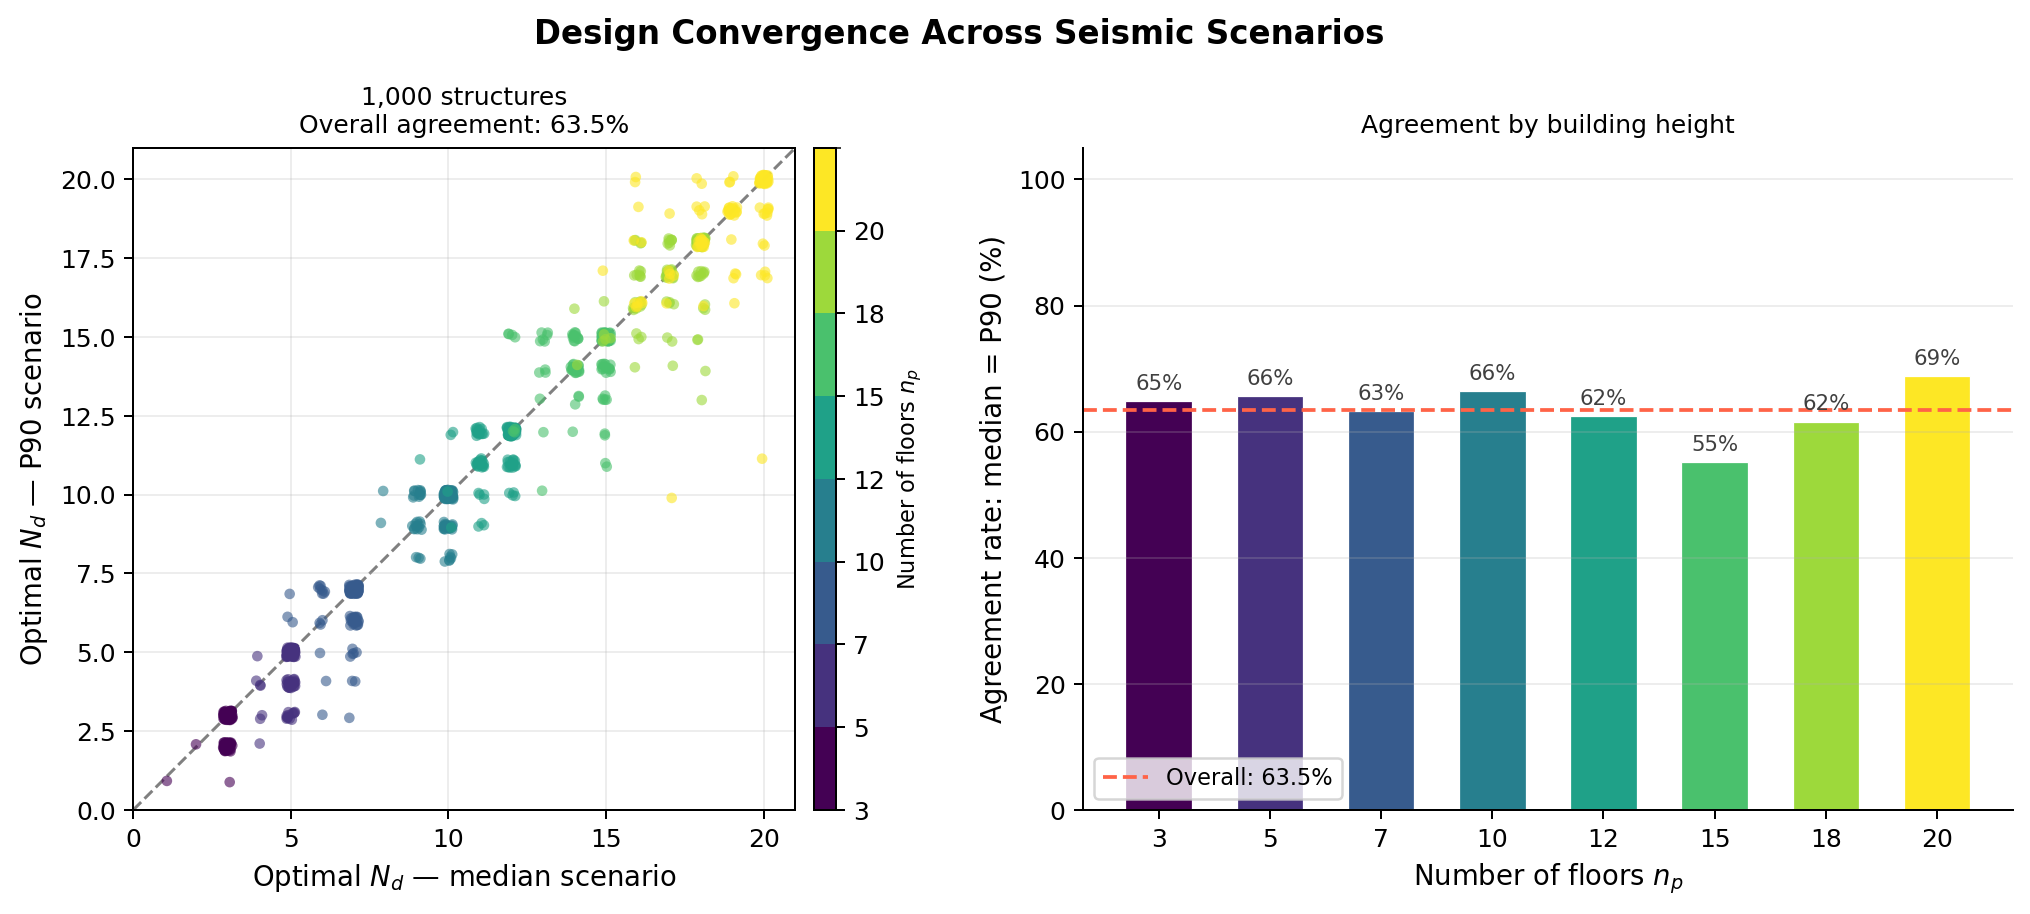
\includegraphics[width=\linewidth]{figs/F8_convergence_extended.png}
\caption{Stability of the optimal damper count $\nd$ across seismic scenarios
for 1{,}000 structures. The left panel compares the optimal $\nd$ under the
typical (median) and conservative (P90) scenarios; points on the diagonal
indicate full agreement, and color encodes building height~$\np$. The right
panel summarizes the exact agreement rate by height group; the dashed line
marks the overall agreement rate (63.5\,\%), with a mean discrepancy of
0.51~stories.}
\label{fig:convergencia}
\end{figure}

%%═══════════════════════════════════════════════════════════════════════════
\section{Discussion}
\label{sec:discussion}
%%═══════════════════════════════════════════════════════════════════════════

\subsection{Coverage Density as the Governing Design Parameter}

Among all design variables, coverage density $\etad$ emerges as the strongest
predictor of $CR_2$ ($\rho = -0.73$), and this dominance holds consistently
across all eight seismic records (\cref{sec:results:decreciente}). Translating
the 80\,\% maximum-gain threshold into actionable guidance, the analysis
recommends $\etad \geq 0.85$ for mid- and high-rise frames (6--20~stories)
and $\etad \geq 0.95$ for low-rise frames (3--5~stories). These thresholds
mark the point beyond which adding more dampers returns only marginal
improvement---a directly applicable cost-effectiveness criterion for
preliminary RFD deployment decisions.

\subsection{Interaction Between Friction Moment and Coverage}

Coverage density determines how many floors are instrumented, but the friction
moment $\Mf$ governs how much each device contributes. The two variables are
not independent: \cref{fig:mapa_calor} shows that at intermediate coverage
levels, doubling $\Mf$ at a fixed device count yields $CR_2$ reductions
comparable to adding two additional instrumented floors. In other words, a
designer who cannot install more devices can still recover much of the
performance gain by increasing the friction moment of the existing ones---up
to a point. Beyond $\etad \approx 0.75$, the sensitivity to $\Mf$ diminishes
and coverage becomes the binding constraint again.

This complementarity is precisely the kind of nonlinear interaction that
marginal correlation analysis misses and that motivates the ensemble ML
approach. As for the magnitude of $\Mf$, \citet{Jarrahi2020sdee} reported
an effective range of 81--439\,kN$\cdot$m for six dampers in a 10-story
steel moment-resisting frame (SMRF), and \citet{Ponce2026} identified
350--450\,kN$\cdot$m as the optimal range for the same structural type under
a probabilistic framework. The range found here, $\Mf \in [300,\,460]$\,kN$\cdot$m
(median 400\,kN$\cdot$m), sits squarely within both references, lending
independent cross-validation to the ML-identified optimum across a much
broader set of structural configurations.

\subsection{Comparison with Jarrahi et al.\ (2020): Energy vs.\ Displacement Criteria}

\citet{Jarrahi2020sdee} studied RFD performance in a 10-story SMRF and
reported that the energy dissipation objective saturates at
$\etad \approx 0.60$, the point at which frame yielding is effectively
suppressed. The present study finds saturation at $\etad \approx 0.85$---
25 percentage points higher. The discrepancy is not a contradiction; it
reflects the fact that the two studies measure different things. An
energy-based criterion asks: \emph{when does the frame stop yielding?}
The $CR_2$ criterion asks: \emph{when do displacement, acceleration, and
base-shear demands stop improving?} Because non-structural acceleration
demands ($R_2$) and base shear ($R_3$) continue to respond to additional
coverage beyond the yielding threshold, $CR_2$ detects saturation later.
The two thresholds are therefore best understood as complementary performance
levels:
\begin{itemize}
    \item $\etad \geq 0.60$: structural damage prevention, sufficient when
          the design objective is to protect load-bearing elements
          \citep{Jarrahi2020sdee};
    \item $\etad \geq 0.85$: serviceability control, required when the
          design must additionally limit acceleration demands on non-structural
          components, equipment, and building occupants.
\end{itemize}
A practitioner can use the first threshold as a minimum bound and the second
as the target when full performance-based objectives are in play.

\subsection{Robustness Across Scenarios}

\citet{Jarrahi2020jbe} and \citet{Jarrahi2020sdee} optimized RFD
configurations against individual seismic records, leaving open the question
of whether a design tuned to one record remains effective under a different
excitation. The multi-record framework adopted here addresses this directly:
by evaluating each configuration against eight historical accelerograms and
summarizing performance through P10, median, and P90 statistics, the
resulting recommendations are inherently robust to uncertainty in ground
motion selection. The convergence results (\cref{fig:convergencia}) confirm
this robustness quantitatively---63.5\,\% exact agreement and a mean
discrepancy of only 0.51~stories between median and P90 recommendations---
showing that a single optimization pass against the typical scenario is
sufficient to identify a design that also performs well under severe demand.

\subsection{Limitations}

Five limitations bound the scope of the present conclusions.
First, the structural models are idealized elastic shear frames; frame
yielding and its interaction with the RFD response are not captured, so
the recommendations apply to demand levels where the frame remains elastic
or quasi-elastic. Second, the eight accelerograms, while geographically
diverse, may not represent all relevant tectonic environments, particularly
subduction zones with long-duration ground motions. Third, model validation
relies on cross-validation; an independent hold-out test set would provide a
more rigorous bound on generalization error. Fourth, a uniform $\Mf$ is
assumed across all devices in a structure; floor-specific friction moments
could further improve performance but would substantially expand the design
space. Fifth, no installation cost function is included, so the
recommendations maximize seismic performance without penalizing the number
of devices---an economic optimization layer remains as future work.

%%═══════════════════════════════════════════════════════════════════════════
\section{Conclusions}
\label{sec:conclusions}
%%═══════════════════════════════════════════════════════════════════════════

The following main conclusions are drawn from the analysis of
$\approx$434,000 nonlinear time-history simulations over 1,000 diverse
structural configurations and eight real seismic records:

\begin{enumerate}

\item \textbf{ML surrogate model accuracy.}
XGBoost and Random Forest achieved $\Rsq$ of 0.92--0.93 for $\CR{med}$
and $\CR{P10}$, and 0.84 for $\CR{P90}$. Ensemble models reduced prediction
error by $\approx$49\,\% relative to linear baselines, quantifying the
nonlinear structure of the design--performance relationship.

\item \textbf{Diminishing-returns threshold: $\etad \approx 0.85$.}
Within-structure analysis reveals that 80\,\% of the maximum $CR_2$ reduction
is reached at $\etad \approx 0.85$ for mid- and high-rise frames (6--20~stories)
and at $\etad \approx 0.95$ for low-rise frames (3--5~stories). These
thresholds provide practical cost-effectiveness criteria for RFD deployment.
Complementarily, the optimal $\Mf$ identified by ML concentrates in
[300,\,460]\KM (median 400\KM); for $\etad \geq 0.75$, $CR_2$ is relatively
insensitive to the specific $\Mf$ value within [200,\,500]\KM, making
coverage fraction the most critical design parameter.

\item \textbf{Comparison with the energy-based threshold of Jarrahi et al.}
\citet{Jarrahi2020sdee} reported saturation of the energy objective at
$\etad \approx 0.60$ (structural yielding eliminated). The displacement-based
criterion here finds saturation at $\etad \approx 0.85$, 25 percentage
points higher. The difference is explained by the greater sensitivity of
$CR_2$ to displacement and acceleration demands that persist beyond the
yielding threshold. The two criteria describe complementary performance
levels: $\etad \geq 0.60$ targets structural damage prevention;
$\etad \geq 0.85$ additionally controls serviceability.

\item \textbf{Robustness across scenarios.}
63.5\,\% of structures receive exactly the same $\nd$ recommendation under
the median and P90 scenarios, with a mean discrepancy of 0.51~stories in the
remaining cases. A design optimized for the median scenario provides
near-optimal protection across the full seismic variability of the
eight-record ensemble.

\item \textbf{Future work.}
Three extensions of the NSD-LCP-PSOR engine itself are of immediate interest.
First, incorporating soil--structure interaction (SSI) into the formulation
would allow the compliance of the foundation to modify the effective input
motion and the frequency content seen by the dampers---an effect that can be
decisive for soft soils and tall buildings. Second, extending the shear-frame
model to three-dimensional frames would capture torsional coupling and
bidirectional excitation, which are absent in the current planar idealization
and may shift the optimal placement patterns for asymmetric buildings. Third,
replacing the elastic frame elements with nonlinear (inelastic) formulations
would enable the simulation of high-intensity scenarios where frame yielding
interacts with the RFD response, which is the primary source of epistemic
uncertainty in the present results. Beyond the simulation engine, future work
should address floor-specific $\Mf$ distributions, installation cost
constraints, broader seismic record suites covering different tectonic
environments, and integration of the trained surrogate models into an
interactive design tool.

\end{enumerate}

%%═══════════════════════════════════════════════════════════════════════════
\section*{CRediT Author Contribution Statement}

\textbf{E.~Ponce}: Conceptualization, Methodology, Software, Formal Analysis,
Investigation, Validation, Data Curation, Visualization, Writing -- Original Draft.
\textbf{H.~Yañez-Godoy}: Conceptualization, Supervision, Writing -- Review \& Editing.

\section*{Declaration of Competing Interests}

The authors declare that they have no known competing financial interests or
personal relationships that could have appeared to influence the work reported
in this paper.

\section*{Funding}

This research did not receive any specific grant from funding agencies in the
public, commercial, or not-for-profit sectors.

\section*{Acknowledgements}

The first author gratefully acknowledges the financial support provided by the
Secretaría de Ciencias, Humanidades, Tecnología e Innovación (SECIHTI, Mexico)
through a master's scholarship. The authors also acknowledge the institutional
support of the Universidad Autónoma de Querétaro (UAQ, Mexico) and the Institut
de Mécanique et d'Ingénierie (I2M, UMR CNRS 5295), University of Bordeaux,
France.

\section*{Data and Code Availability}

The simulation pipeline (Phases 1--4), the aggregated ML dataset
($\approx$50,000 configurations), and the LHS random seed are publicly
available at \url{https://zenodo.org/record/XXXXXXX} (DOI:
10.5281/zenodo.XXXXXXX). The repository includes all scripts required to
reproduce the figures and tables reported in this paper. Data will be
made fully available upon acceptance of the manuscript.

\section*{Declaration of Generative AI and AI-Assisted Technologies in the
Writing Process}

During the preparation of this work the authors used Claude (Anthropic) in order
to assist with translation from Spanish to English and language style correction.
After using this tool, the authors reviewed and edited the content as needed and
take full responsibility for the content of the publication.

%%═══════════════════════════════════════════════════════════════════════════
\bibliographystyle{elsarticle-harv}
\bibliography{references}

\end{document}
